%Template by Mark Jervelund - 2015 - mjerv15@student.sdu.dk

\documentclass[a4paper,10pt,titlepage]{report}

\usepackage[utf8]{inputenc}
\usepackage[T1]{fontenc}
\usepackage[english]{babel}
\usepackage{amssymb}
\usepackage{amsmath}
\usepackage{amsthm}
\usepackage{graphicx}
\usepackage{fancyhdr}
\usepackage{lastpage}
\usepackage{listings}
\usepackage{algorithm}
\usepackage{algpseudocode}
\usepackage[document]{ragged2e}
\usepackage[margin=1in]{geometry}
\usepackage{color}
\usepackage{datenumber}
\usepackage{venndiagram}
\usepackage{chngcntr}
\setdatetoday
\addtocounter{datenumber}{0} %date for dilierry standard is today
\setdatebynumber{\thedatenumber}
\date{}
\setcounter{secnumdepth}{0}
\pagestyle{fancy}
\fancyhf{}

\newcommand{\Z}{\mathbb{Z}}
\lhead{Computer Architecture (DM548))}
\rhead{Mark Jervelund (Mjerv15)}
\rfoot{Page  \thepage \, of \pageref{LastPage}}
\counterwithin*{equation}{section}

\begin{document}
\renewcommand{\thepage}{\roman{page}}% Roman numerals for page counter
\tableofcontents
\newpage
\setcounter{page}{1}
\renewcommand{\thepage}{\arabic{page}}
\section{Course description}
To describe the services an operating system provides to
users, processes, and other systems\\
To discuss the various ways of structuring an operating
system\\
To explain how operating systems are installed and
customized and how they boot\\
\newpage
\section{Question 1 - Operating System Services - ch 2}
%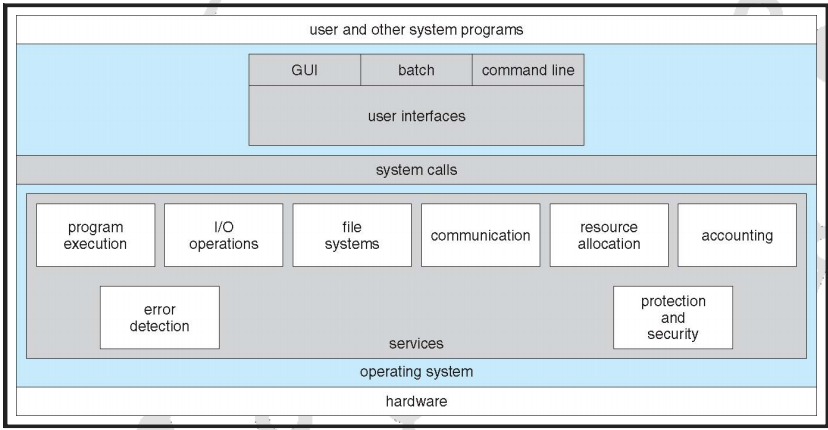
\includegraphics[scale=0.5]{Picture1.png}
User interfaces = Command-Line (CLI), Graphics User Interface (GUI), Batch \\


\subsection{Keywords}
1.) Short introduction \\
\hspace{10mm}explain the 3 types of interfaces. GUI, CLI, and batch\\
\hspace{15mm}Explain pros and cons\\
\hspace{20mm}CLI - Requires more knowlage about how it works. \\
\hspace{20mm}GUI - More intuative and easier to use \\
\vspace{5mm}


2.)

How you communicate between OS and programs,\\
\hspace{10mm}System calls - How do you call them, how to use them. parameters etc. \\
\hspace{15mm} Check file with the list of system calls \\
\hspace{15mm} Find the file corresponding to the system call.\\
\hspace{15mm} puts the parameters\\
\hspace{20mm} using registers\\
\hspace{20mm} stores in block and address of block is passed to the function as a parameters\\
\hspace{20mm} places or pushed on the stack and POPed by the operating system.\\
\vspace{5mm}


3*)
Process communications\\ \textcolor{red}{TODO:more} \\
\hspace{10mm}Message parsing and shared memory \\ 
\hspace{15mm} pro/cons \\
\hspace{10mm} shared memory, uses less space as memory is only copied if it gets changed.\\
\hspace{10mm} Message parsing, \textcolor{red}{TODO} \\
\hspace{15mm} Either directly between two processes or to a mailbox(?)  \textcolor{red}{TODO:Please confirm}
\vspace{5mm}


4*) 
OS structure \\ 
\textcolor{red}{TOOD:CHECK} \\


\hspace{10mm}	Simple structure \\
\hspace{15mm}    	There is no control, applications can talk directly to hardware and the kernel.\\


\hspace{10mm}    Layered \\
\hspace{15mm}    	There are multiple layers,the user can only talk to the the applications,the applications can only talk to the operating system API, and only the operating system can call to the kernel \\
\hspace{15mm}        User->Application->OS->Hardware \\

\hspace{10mm}	Micro-kernel\\
\hspace{15mm}		Move as much as the kernel as you can into user-space. User mode applications can communicate via the kernel.
    
\hspace{10mm}   Modules \\
\hspace{15mm}		Indivisdual modules that can be loaded and unloaded into the kernel, so provide some kind of use.
                
\hspace{10mm}    Hybrid-systems \\
\hspace{15mm} Most modern operating systems are not one pure model, 



\vspace{5mm}


5)
Debugging\\
\hspace{10mm}What can we do when something goes wrong? \\
\hspace{15mm}	Log files, data dumps, tracing tools. Windows task-manager essential, Linux has the top/htop command \\

\vspace{5mm}


6)
Boot-loaders, How does the os know where to find the boot-loader, kernel, etc. \\




\subsection{Questions from lecture}
What is a system call.\\
\hspace{10mm} Programming interface to the services provided by the operating system \\ \vspace{5mm}


What groups of system calls are there. \\
\hspace{10mm}File manipulation, process control, security and protection, communication, I/O device manipulation \& information management\\ \vspace{5mm}


why would you use a system call API.\\
\hspace{10mm}Ease of use, Reduce failure, reuseability/portability \\ \vspace{5mm}


What ways are there to pass parameters to the OS.\\
\hspace{10mm} Stack + reference, register, memory -> send reference \\  \vspace{5mm}


How can an operating system be structured(architecture wise)\\
\hspace{10mm} Layered structure, module based, micro-kernel \& hybrid systems\\ \vspace{5mm} 


what code is first read when you turn on your computer\\
\hspace{10mm}Bootstrap code located in EPROM \\ \vspace{5mm}





\newpage
\section{Question 2 - Process Concept and Multi threaded Programming - ch 3 \& 4}
Process control block. \\ Diagram on slide 3.7
\vspace{5mm}

\subsection{Keywords}
1) Introduction - \\
\hspace{10mm}	What is a process. \\
\hspace{10mm}	Process control block. \\
\hspace{15mm}	State \\
\hspace{15mm}	Process number \\
\hspace{15mm}	Program counter \\
\hspace{15mm} 	Registers \\
\hspace{15mm}	Memory limits \\
\hspace{15mm} 	Files descriptors (active files ) \\
\hspace{15mm} 	.... \\
\vspace{5mm}


2) Process scheduling - \\
\hspace{10mm}	CPU \& I/O burst \\
\hspace{10mm}	Short, medium \& long schedulers.\\
\hspace{15mm}   Short - from ready, to running.
\hspace{15mm}	Medium - medium running to waiting. and waiting to ready (context swap)
\hspace{15mm}	Long - Loads jobs into the new/ready queue from a work queue.

\hspace{10mm} Schedulers.\\
\hspace{15mm} First come first service\\
\hspace{15mm} Shortest job first \\
\hspace{15mm} Shortest time remaining first \\
\hspace{15mm} Round robin\\
\hspace{15mm}give each process the same amount of time and loop over them until they're done. circular queue\\
\vspace{5mm}


3) Context switch.\\
\hspace{10mm} Saves current state of the process and stores it, when the process waits for I/O.\\
\vspace{5mm}
4) Interprocess communication - \\
\hspace{10mm}	Message parsing \\
\hspace{15mm}  	The processes can communicate with each other without resorting to shared variables	\\
\hspace{15mm} 	This is done using by using a IPC facility that has two operations. a send and a receive operation.
\hspace{15mm} 	If eg. P and Q wish to communicate they'll need to first establish a link between them, and then exchange the message via send/receive.
\hspace{15mm} Direct and indirect(mainbox with id)


\hspace{10mm}	Shared memory \\
\hspace{15mm}	Fixed shared memory segment \\
\hspace{15mm}\textcolor{red}{TODO:}
\vspace{5mm}

5) Communication-\\
\textcolor{red}{TODO:}
\hspace{10mm}	Client/server\\
\hspace{10mm}	RPC\\
\hspace{10mm}	Socket \\
\hspace{10mm}	Pipes\\
\vspace{5mm}


Concurrency /parallel - \\
\textcolor{red}{TODO:}
\hspace{10mm} Whats the difference\\
\vspace{5mm}



7) Multicore programming \\
\textcolor{red}{TODO:}
\vspace{5mm}

8) Multitreading \\
\hspace{10mm} Many to one \\
\hspace{10mm} One to One \\
\hspace{10mm} Many to Many \\	
\vspace{5mm}

9) Thread libraries \\
\hspace{10mm} Boost (maybe builds on pthread) \\
\hspace{10mm} Pthread \\
\hspace{10mm} javathread \\
\hspace{10mm} Winthread \\
\vspace{5mm}

10) Implicit Threading \\
\textcolor{red}{TODO:}
\vspace{5mm}

11) Threading Issues \\
\textcolor{red}{TODO:}
\vspace{5mm}





\newpage
\subsection{Questions from lecture}
What state can a process by in?\\
\hspace{10mm}New.\\
\hspace{10mm}Ready.\\
\hspace{10mm}running.\\
\hspace{10mm}waiting.\\
\hspace{10mm}terminated.\\
\vspace{5mm}




What is a process control block?\\
\hspace{10mm}A block where the OS store information about a program.\\ 
\hspace{10mm}Used for content switching and stores the following information:\\
\hspace{20mm}Process state\\
\hspace{20mm}Process number\\
\hspace{20mm}Process counter\\
\hspace{20mm}Registers\\
\hspace{20mm}Memory limits\\
\hspace{20mm}List of open files\\


\vspace{5mm}
Describe ways to do IPC\\
\hspace{10mm}Message parsing and memory shearing. \\




\vspace{5mm}
What is the difference between a process and a thread\\
\hspace{10mm}A process is a thing we need to execute, and thread is a subtask of a process.\\


\vspace{5mm}
What advantages is there when using threads?\\
\hspace{10mm}Threading lets you work on multiple cores at the same time, therefor letting you run a job faster.\\


\vspace{5mm}
Difference between parallelism and concurrency?\\

\hspace{10mm}	Parallelism - same task spread on multiple threads\\
\hspace{10mm}	Concurrency - program running with multiple threads\\
\hspace{10mm}  	We can have Concurrency without Parallelism but not the other way around\\



\vspace{5mm}
What are the most common API's for user level threads\\
\hspace{10mm} Boost (maybe builds on pthread) \\
\hspace{10mm} Pthread \\
\hspace{10mm} Java thread \\
\hspace{10mm} Winthread \\
\vspace{5mm}



What are the implicit threading methods.\\
\hspace{10mm} Thead pools \\
\hspace{10mm} Openmp \\
\hspace{10mm} Grand Central Dispatch \\

\newpage

\section{Question 3 - Process Scheduling - ch 5}
Scheduling types\\
FCFS - unstable wait time.\\
Shortest job first. optimal. gives minium wait time, but only usable for long time sheduling.\\
\vspace{5mm}
\subsection{Questions from lecture}
1. When is it Relevent for the scheduler to take  decision.\\
\hspace{10mm}When a new process queued, and a new processes is started.\\
\hspace{10mm}4 cases\\
\hspace{20mm}when a process running state to waiting.\\
\hspace{20mm}when a process terminates.\\
\hspace{20mm}When a process is queued\\
\hspace{20mm}When a process goes from waiting to ready\\

\vspace{5mm}

What is dispatch latency.\\
\hspace{10mm} time it takes for a interupting process to become active \\
\hspace{10mm} move memory and registers from the running task, move new tasks there and start it \\
\vspace{5mm}

What scheduling ctiteria can we use.\\
\hspace{10mm} maximize CPU util, low latency for take critical jobs jobs.\\
\hspace{10mm} runtime, priority, CPU bound, I/p bound \\
\vspace{5mm}

Describe the scheduling algortirhms: FCFS, SJF, Shortest remaining time fist, RR.\\
\hspace{10mm} First come first servce\\
\hspace{10mm} Shortest job first \\
\hspace{10mm} Shortest time remaining first \\
\hspace{10mm} Round robin\\
\hspace{10mm}give each process the same amount of time and loop over them until they're done. circular queue\\
\vspace{5mm}


Describe priority schduling and aging\\
\hspace{10mm} The longer it has been in the queue the higher the priority the job has\\
\vspace{5mm}

What is the difference betweeen asymmetric and symmetric multiprocessing\\
\hspace{10mm} Asymmmetric means tasks wont wait for other things \\
\hspace{10mm} Not all processes has the some capapicities\\
\hspace{10mm} All the kernals can do the same.\\ 
\vspace{5mm}

What is a memory stall\\
\hspace{10mm} Waiting for memory ? \\
\vspace{5mm}



What is the difference between soft and hard real-time systems.\\
\hspace{10mm} Soft -  Don't time life critital systems while hard real time systems have.\\
\vspace{5mm}




Describe rate montonic scheduling and earlist deadline scheduling\\
\hspace{10mm} rate montonic scheduling - Schedule jobs in intervals, like a, b, c.\\
\hspace{10mm} earlist deadline scheduling - Schedule the process with the first deadline first.\\
\vspace{5mm}


\subsection{Keywords}
1. Introduktion\\
what is CPU bound\\
what is I/O bound\\
explain as shortterm, medium term, and long term\\
2. Criterias\\
What do we want to take a look at as I/O bound, like what can we do to get a better CPU Util\\
3. Algorithmer \\ 
Explain FCFS, SJF, etc.\\
starvation etc. \\
4. Multi processer scheduling.\\
Single queue, queue per core, shared queues\\
5. Realtime schduling\\

6. Examples\\
\newpage
\section{Question 4 - Synchronization - Lecture 5}

\subsection{Questions from lecture}

Describe the terms "race condition" and "Critical section"\\

\hspace{10mm} When two proceses want to access a shared resource. that may be unstable if its done in a \\ \hspace{10mm} non-locked way\\
\hspace{10mm} 
Race condition is when multiple processes/threads are competing about the same resources and \\ \hspace{10mm}  a undesired output may happen. \\


\hspace{10mm}  Critical section is a section of code that sensitive to race conditions.\\

What should a solution to the critical section satisfy \\
\hspace{10mm}  Mutual exclution, progress, and \\
\hspace{10mm}  that only one thread can be active in the critical section at the time. \\

What is preemptive vs. non preemptive \\

\hspace{10mm}  preemptive is the act is  temporarily interrupting a process\\

\hspace{10mm}  non-preemptive -  When a process enters the state of running, the state of that process is not \\ \hspace{10mm} deleted from the scheduler until it finishes its service time.\\

Describe "test and set" and "compare and swap". \\

\hspace{10mm}  Two different ways of implementing a mutex lock, that are garenttted to be excuted in an atomic \\ \hspace{10mm} way.\\

\hspace{10mm} Test and set - \\

\hspace{10mm}  Compare and swap can only be used by one function, its checks for a codition and sets swaps \\ \hspace{10mm}  two value if the condition is met.\\ 

What is a mutex and a semaphore \\

\hspace{10mm}  a Mutex lock is a lock where only the process holding the lock is allowed to perform actions in \\ \hspace{10mm}  	the locked section. \\
\hspace{10mm}  A mutex contains a boolean and is acquired and released.\\


\hspace{10mm}  A binary semaphore is the same as a mutex. \\

\hspace{10mm}  a counting semaphore is when the lock uses a counter if multiple processes can be active within \\
\hspace{10mm}  the lock. \\


Describe some classic problems of synchronization. \\

\hspace{10mm}  Readers writers problems.\\
\hspace{10mm} dining philosopher problem. \\


What is a monitor \\
\hspace{10mm}  We can put functions into the monitor and only one process can be active within the monitor \\
\hspace{10mm} at the time, else the process will have to wait in the queue.






\subsection{Keywords}
1. Introduction\\
2. Critital section\\
3. software solution to critical section\\
4. hardware solutions to critical section\\
5. mutex lock\\
6. semaphore lock\\
7. monitors\\
8. spinlock\\
9. alternative solution\\
10. exemples\\

\newpage
\section{Question 5 - Deadlocks - Lecture 6}
\subsection{Objectives}
To develop a description of deadlocks, which prevent sets of concurrent
processes from completing their tasks\\
To present a number of different methods for preventing or avoiding
deadlocks in a computer system\\
\subsection{Notes}
\subsubsection{What is a deadlock}
4 things have to hold for a deadlock to happen, these are Mutual exclusion
Hold and wait
No preemption
Circular wait
\\
Mutual exclusion\\
\hspace{10mm} Only one process at a time can use a resource\\
Hold and wait\\
\hspace{10mm} A process holding at least one resource is waiting to acquire additional
resources held by other processes \\
No preemption\\
\hspace{10mm} A resource can be released only voluntarily by the process holding it, after
that process has completed its task \\ 
Circular wait\\
\hspace{10mm} There exists a set {P0 , P1 , … , Pn } of waiting processes such that P0 is waiting
for a resource \\
\hspace{10mm} that is held by P1 , P1 is waiting for a resource that is held by
P2 , … , Pn–1 is waiting for a \\
\hspace{10mm}resource that is held by Pn, and Pn is waiting for a
resource that is held by P0. \\
\vspace{2mm} 
\hspace{10mm}We have a circle of tasks waiting for each other.
\\
\subsubsection{How can a deadlock be detected}

\subsubsection{Graph detection}
Deadlocks can be detected by looking for cycles in a graph, this doesn't mean that we have a deadlock, but it means we have a risk of there being one.\\
no cycles  $\rightarrow $ no deadlock
If graph contains a cycle $\rightarrow $ \\
\hspace{10mm} if only one instance per resource type, then deadlock
\\
\hspace{10mm} if several instances per resource type, possibility of deadlock

\subsubsection{Methods for handling deadlocks}
1. Ensure that the system will never enter a deadlock state\\
2. Allow the system to enter a deadlock state and then recover\\
3. Ignore the problem and pretend that deadlocks never occur in the system; \\
\hspace{10mm} used by most operating systems
\subsubsection{Deadlock prevention}
\textbf{Mutual exclusion }- 
\\ 
\hspace{10mm} not required for sharable resources; must hold for
nonsharable resources
\\
\textbf{Hold and wait} - \\
\hspace{10mm}
must guarantee that whenever a process requests a resource, it does not
hold any other \\
\hspace{10mm} resources.
\\
\hspace{10mm}
Request all resources up front before execution. (all or none)\\

\textbf{No Preemption} - \\
\hspace{10mm}If a process that is holding some resources requests another resource that
cannot be immediately \\
\hspace{10mm}allocated to it, then all resources currently being held
are released\\
\hspace{10mm}Preempted resources are added to the list of resources for which the process
is waiting\\

\hspace{10mm}Process will be restarted only when it can regain its old resources, as well as
the new ones that \\
\hspace{10mm}it is requesting\\

\textbf{Circular Wait} \\
\hspace{10mm}Impose a total ordering of all resource types, and require that each process
requests resources in \\
\hspace{10mm} an increasing order of enumeration.\\
\subsubsection{Deadlock avoidance}
Requires that the system has some additional a priori information available \\
Simplest and most useful model requires that each process declare the
maximum number of resources of each type that it may need
\\
\vspace{10mm}

The deadlock-avoidance algorithm dynamically examines the resourceallocation
state to ensure that there can never be a circular-wait condition
\\
Resource-allocation state is defined by the number of available and allocated
resources, and the maximum demands of the processes. \\

\subsubsection{Avoidance algorithms}
Single instance of a resource type $ \rightarrow $  Use a resource-allocation graph \\
Multiple instances of a resource type $ \rightarrow $ Use the bankers algorithm\\


\subsection{Questions from lecture}
which 4 conditions most hold for a deadlock\\
\hspace{10mm} and describe them \\
\hspace{10mm} mutual exclusion\\
\hspace{20mm} Two processes lock each other out due to interrupt  \\
\hspace{10mm} hold and wait\\
\hspace{20mm} Processes is waiting for resources to be released by other process \\
\hspace{10mm} circular wait\\
\hspace{20mm} two or more processes are waiting for each other to release resources \\
\hspace{10mm} no pre-emption\\
\hspace{20mm} cant remember \\


Describe the resource graph\\
\hspace{10mm} Graph the shows the dependency of resources and processes \\


What methods are there to handle deadlocks \\
\hspace{10mm} avoid deadlock \\
\hspace{10mm} allow deadlocks and recover \\
\hspace{10mm} ignore them  \\


What is a safe state \\
\hspace{10mm} A state where deadlocks cant occur \\


Describe the general idea of bankers algorithm \\
\hspace{10mm} each process says how many resources they require, and the scheduler assigns the so no deadlocks occur\\


How can a deadlock be detached \\
\hspace{10mm} multiple processes are waiting for each other, and this can be detached with a resource graph \\


How can you recover from a deadlock\\
\hspace{10mm} kill processes that are in the deadlock until its resolved. \\

If you don't feel super comfy with deadlocks. talk about locks, and synchronization.
\newpage
\subsection{Keywords}
1. Introduction\\
\hspace{10mm} What is a deadlock\\
\hspace{10mm} 4 conditions \\
\hspace{20mm} mutual exclusion, hold and wait, circular wait, and no pre-emption \\
\hspace{20mm} Show a small example, resource graph \\


2.  How to handle a deadlock \\
\hspace{10mm} Prevent and avoid \\
\hspace{10mm} recover \\
\hspace{15mm} Start killing tasks that are in the deadlock until its resolved \\
\hspace{10mm} Ignore \\
\hspace{15mm} Let the user handle it \\


3. How to avoid a deadlock \\
\hspace{10mm} How to avoid the 4 conditions \\
\hspace{15mm} If we can change one we can avoid \\


4. avoiding a deadlock \\
\hspace{10mm} bankers algorithm \\
\hspace{10mm} resources graphs \\
\hspace{10mm} what is the criteria for that they are in safe and unsafe states \\

5. Deadlock detection  \\
\hspace{10mm} resources graph detection \\


6. why do we want to avoid deadlocks\\
\hspace{10mm} give examples on when to avoid deadlocks.

7. Recover \\
\hspace{10mm} Show some algorithms on how to avoid a deadlock \\

8. Examples \\
%



\newpage
\section{Question 6 - Memory Management Strategies - ch 8}
\subsection{notes}
\subsubsection{Introduction}
Detailed description of various ways of organizing memory hardware\\
Various memory-management techniques, including paging and segmentation \\
To provide a detailed description of the Intel Pentium, which supports both pure segmentation and
segmentation with paging \\

\subsection{Questions from lecture}
\textbf{In which stages can address binding happen}.\\
\hspace{10mm} compile time \\
\hspace{15mm} If memory location known a priori, absolute code can be generated; must recompile code if starting location changes \\



\hspace{10mm} Load time\\
\hspace{15mm} Must generate relocatable code if memory location is not known at compile time



\hspace{10mm} Execution time \\
\hspace{15mm} Binding delayed until run time if the process can be moved during its execution from one memory segment to another \\

\vspace{5mm}

\textbf{What is an relocation register}\\
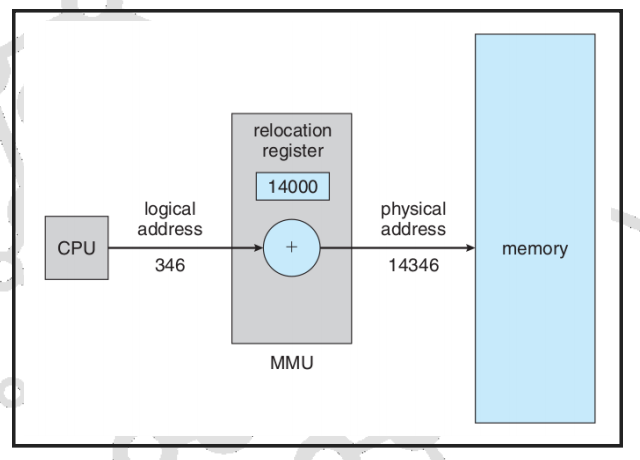
\includegraphics[scale=0.5]{relocation.png}
offset

\vspace{5mm}

\textbf{describe dynamic loading and dynamic linking} \\
\hspace{10mm}dynamic loading is when we load the libraries after load time\\
\hspace{10mm}dynamic linking is when we set the offset after the program have been loaded \\ 
\vspace{5mm}

\textbf{describe swapping and the back stores role} \\
\hspace{10mm} Swapping is when you store memory pages on cold storage due to low/no remaining memory (extremely slow)\\
\hspace{10mm} back stores role \\


\vspace{5mm}
\textbf{describe some algorithm for the dynamic storage-allocation problem} \\
\hspace{10mm} First Fit \\
\hspace{10mm} Worst Fit \\
\hspace{10mm} Best Fit \\

\vspace{5mm}
\textbf{difference between external and internal fragmentation}\\
\hspace{10mm} Internal fragmentation is when there is unused memory within a process allocation \\
\hspace{10mm} external is when there is unused memory between two processes \\

\vspace{5mm}
\textbf{describe segmentation and paging.}\\
\hspace{10mm} segmentation is when you segmentation a program into data, execution code, etc  \\
\hspace{10mm} paging is when you split a program into pages, so there is no external fragmentation, but only internal on the last page of the program.\\


\subsection{Keywords}

Introduction\\
\hspace{10mm} The background\\
\hspace{15mm} How do we access our memory \\
\hspace{15mm} Address binding \\
\hspace{15mm} paging, the different types that we have \\
Swapping \\
\hspace{10mm} How do we swap processes between the memory and the disk \\
Contigious memory allocation \\
Segmentation \\
Paging \\
\hspace{10mm} hierarchical \\
Page table (TLB) \\
Pros/cons \\
Case examples \\






\section{Question 7 - Virtual memory - ch 9}
\subsection{notes}


\subsubsection{Introduction}

\subsubsection{Virtual address space}

\subsubsection{Demand pages}
Means we wont have to load all pages into memory, so processes can start faster. this uses a 

\subsubsection{page fault}
Reference to a page that is not in memory, when this happens the OS check is if valid or not, if its not valid the os will throw an exception, and if its valid the page is loaded into memory, while this is happening the processes is put in a hold state(its a trap) and continued when the page is loaded into memory 
\subsubsection{hardware demand}
page table with valid/invalid\\

\subsubsection{performance of demand paging}

\subsubsection{Page replacement}
\hspace{10mm} first in first out\\
\hspace{10mm} Least recently used\\
\hspace{15mm} can use system clock or a stack with dual pointers, and move it to the top if its used. and always picks the one in button if its used.\\
\hspace{15mm} Needs special hardware, its still slow, due to pointers needing to being changed \\
\hspace{10mm} Second chance \\
\hspace{15mm} clock, first in first out, with a reference bit \\

\hspace{10mm} Least frequently used\\

\hspace{10mm} Most frequently used\\

\hspace{10mm} Optimal page replacement \\
\hspace{15mm}Doesn't exist as we do not know the future. \\
\hspace{15mm}But its good for comparing with other to see how they compare to the optimal.\\

\subsubsection{Page allocation}

\hspace{10mm} Fixed allocation \\

\hspace{15mm} equal allocation \\
\hspace{20mm} dynamic, allocates based on size \\

\hspace{10mm} priority allocation \\

\hspace{15mm} shift memory from low priority to high priority, \\

\subsubsection{Working set}



\subsection{Questions from lecture}

Describe demand paging
Bring pages into memory when it is needed, meaning less I/O, less memory needed and faster response.

Describe copy on write
"Everyone" has a single shared copy of the same data until it's written, and then a copy is made

We fork the file so both the parent and the child are using the same file. when a write happen we copy the file so the thread that child and parent aren't working on the same file

needs rewriting.

Describe the page replacement algorithms

FIFO
First in first out. removed the oldest page in the buffer if requested one isn't there \& and its out of space.


LRU
Least recently used.
Uses past knowledge.
Replaces page that has not been used in the most amount of time 
Associate time of last use with each page

Counter implementation.
    every page has a counter. 

stack implmentation 
    double link form.
    
    
    
Clock
circular clock 



LFU
Least Frequently Used
replaces page with smallest count
Can give problems with some pages with lots of use gets "stuck" in the buffer.

MFU
based on the argument that the page with the smallest count was probably just brought in and has yet to be used

Optimal
    Impossible as we don't know the future.

What is Beladys Anonmaly
Adding more frames can cause more page faults!

Describe trashing
If a process does not have enough pages, it gets a lot of page faults causing a lot of pages to be swapped out, only to be swapped in again.



Describe the working-set model.

The working set model, tries to predict how many frames we need to allocate for a process. at any given time, (it's dynamic)

Explain buddy system
Allocate memory from a fixed size segment.










\subsection{Keywords}
\hspace{10mm} text \\
\hspace{15mm} text \\
\hspace{20mm} text \\

\vspace{5mm}
Introduction \\
\hspace{10mm} What is virtual memory and why do we need it \\
\hspace{10mm} benefits \\

\vspace{5mm}
Denmand paging \\
\hspace{10mm} text \\
\vspace{5mm}

Copy on write \\

\vspace{5mm}

Page replacement algorithms \\
\hspace{10mm}	FIFO \\
\hspace{10mm}	LRU \\
\hspace{10mm}	Optimal \\
\hspace{10mm}   Clock replacement \\

\vspace{5mm}
Allocation of frames \\


\vspace{5mm}


Trashing \\

\vspace{5mm}


Memory mapped files \\

\vspace{5mm}












\section{Question 8 - FILE SYSTEM \& IMPLEMENTING FILESYSTEMS }

May ask things about process control block


\subsection{Notes}
\subsubsection{objectives}

Explain the function and interfaces of file systems\\

Discuss file-system design tradeoffs, including access
methods, file sharing, file locking, and directory structures
Explore file-system protection \\

Describe the details of implementing local file systems
and directory structures\\


Describe the implementation of remote file systems \\

Discuss block allocation and free-block algorithms and
trade-offs
\\
\subsubsection{objectives}


\subsubsection{File control block}
File permissions

File dates (created, access, edited)

add more


\subsubsection{objectives}

\subsection{Questions from lecture}

Describe different directory structures and their implementations 
	single level
		One directory for all users
		
	two level
		one Directory or each user
	tree structure
		infinite number of directories
	General graph
		Link only to files.
	ACYCLIC-GRAPH
		Link

Describe protection measures in file systems

	Creator can set perms on a file.	
	
	Access control list
		Read
		Write,
		Execute
		Append
		Delete
		List
		
	

Describe the layers in a file system

	Application programs.
		Doesnt care about anything
	logical file system.
		Cares about user rights
	file-organization module.
		
	Basic file system.
	I/O control.
		Knows how to talk with the different devices.
	devices.


What does a device driver do?
	
	Translator from file id, to sector on drive.

What does a FCB contain
	
	File permissions
	Size
	Owner, group, ACL(Access control list)
	File dates, created, acess, edited
	File data blocks, or pointers to data blocks (INode)

Describe different methods for locating data for a file
	
	INDEXED ALLOCATION

	LINKED SCHEME
	
	MULTILEVEL INDEX
	
	COMBINED SCHEME\\
	

Describe methods for free space management

	Free list
		Linked list
		

	




\subsection{Keywords}
Intro\\
	i-node\\
	
	
\vspace{5mm}
	
	
Files\\
\hspace{10mm}	Files operations\\
\hspace{10mm}	How you read the files. linked, segmented, random.\\
	
	
\vspace{5mm}
	
	
Directories\\
\hspace{10mm}	How do we know what files and subdirectories are in the directory.\\
	
	
	
\vspace{5mm}
	
Disk structure\\


\vspace{5mm}
File system mounting \\


\vspace{5mm}
File sharing \\

\vspace{5mm}
File access(Protection/permissions)\\
\hspace{10mm} Owner groups\\

\vspace{5mm}
Recovery \\


\vspace{5mm}
Network files \\



\vspace{5mm}
Allocation \\


\vspace{5mm}
Free Space management \\

\hspace{10mm}



	




\section{Question 9 - MASS-STORAGE STRUCTURE \& I/OSYSTEMS }


\subsubsection{Disk}
1-dimensional array of logical blocks\\

Sector 0 is the first sector on the outermost track \\

\subsubsection{Disk - Scheduling}
SSTF
Shortest seek time first.
may cause starvation\\

Scan
Go from lowest index, to highest, and back to lowest, also known as elevator algor.\\



C-scan
Go from lowest index, to highest, and back to lowest without reading.\\



look
Go from lowest index in queue, to highest in queue, and back to lowest in queue without reading.\\
\subsubsection{Disk - Sector}
Header information, Data, ecc code \\






\subsection{Questions from lecture}
	What are the similarities and differences between NAS and SAN \\
		\textcolor{red}{TODO}
	Describe the disc scheduling algorithms; \\
		FCFS, \\
		First come first serve\\
		
		SSTF, \\
		Shortest search first \\
			
		SCAN, \\
		all the way from first sector to last sector and back.\\
		
		LOOK \\
		Like scan by only goes from element to element, and doesn't start from the beginning. \\	
	
		C-Scan, \\
		like scan but doesn't read on the way back \\
		
		
		C-look		
		Like scan  but doesn't read on the way back
		
	Describe sector sparing
		If the drive encounter a sector it can't write to it will then jump and write to a different sector that it has already allocated.
	
	Describe raid and the mechanisms used
	raid 0
		split the data on multiple disks for more speed
	raid 1
	
		copy the data on multiple disk if one fails you wont loose the data.
	raid 2 (Bits striped)
	
	two groups of disk, one group is data, one disk stores the correction code.
	raid 3(bytes striped)
	
		dedicated storage disks and a dedicated parity disk
		
	raid 4(blocks Striped)
	same just with blocks
	
	raid 6(blocks striped, and two distributed parities)
	
	raid 6
	
	raid 10
	
	What is stable storage and how can yo achieve it
	
	Name some of the characteristics of i/o devices
	
	Explain caching, spooling and device reservation
	

\subsection{Keywords}
Introduction
\hspace{10mm} \textbf{Ex} \\
Disk Scheduling 
\hspace{15mm} \textbf{FCFS} \\
\hspace{15mm} \textbf{Look} \\
\hspace{15mm} \textbf{SSFT} \\
\hspace{15mm} \textbf{FCFS} \\



Disk manegment 
\hspace{5mm} \textbf{•} \\


Raid
\hspace{5mm} \textbf{Raid 5/6} \\

I/O

I/O Hardware
	How do to I/O talk to hardware

I/O Streams
	

\section{Question 10 - Virtual Machines }



\subsection{Keywords}
Introduction\\
History\\
Benefits \& features\\
Building blocks\\
Types of VM and implementation\\
Visualization and OS components \\


\subsection{Questions from lecture}
Describe the role of the VMM/hypervisor:\\
	The mange the virtual machines, hardware access, and port forwarding, and such, may only do virtual switches, and more.\\

	


What is an emulator\\
	Program that emulates a different operating system or set of hardware.\\


Name some of the benefits of virtualisation\\
	the processes are separated within the same hardware, and you can run multiple different different operating systems on the same hardware.\\
		Snapshots\\
	use hardware more efficiently\\
	Live migration\\


Describe the "trap and emulate" and "binary translation"\\
	We don't want the user to access the kernel mode on the hardware.\\
	
	So the VMM does all the kernal operations, its just very expensive.\\

Why are nested page tables used\\
	Because each VM has its own memory.\\
		

How is live-migration preformed\\
	1. create new vm on new host\\
	2. move read only pages to new host\\
	3. move read/write pages to new host\\
	4. move dirty pages to new host, and check if there are changes to read/write pages and move those.\\
	5. pause the vm, move the last pages, and point network traffic to new host. \\
	6. shut down old vm. \\



\section{Question 11 - System Protection}



\subsection{Keywords}

Introduction \\
Domains \\
	access matrix \\
Revocation of access rights.\\
capability based system\\
	Need to know \\
Language based protection\\
Types of attacks \\



\subsection{Questions from lecture}

Describe how an access matrix is used and what it contains \\


How can you implement the access matrix \\

What security measure levels should you handle\\

Describe the principles in the following attacks: stack and buffer overflow, virus, trap door.\\

Describe differences between symmetric and asymmetric cryptology\\

What is an authenticator\\


\section{Question 12 - System Security }



\subsection{Keywords}

Introduction \\
Types of attack \\
	Trojan horse \\
	logic bomb \\

symmetrical and asymmetrical encryption \\
	1 key vs 2 key\\
	b64 vs rsa \\
	RSA \\

User authentication \\
	How to store passwords(not everyone should have access). \\
	Firewalls \\
	

\subsection{Questions from lecture}

























\newpage
\section{Exercise}
\subsection{Lecture 2 - Exercise}
\subsubsection{3.1}
3.1 Describe the differences among short-term, medium-term, and long-term scheduling.\\
Use as much CPU time as possible \\
\textbf{Short - Takes a job from rready queue and starts it}\\
\textbf{Medium - Remove Job from active until IO/wait is over. and puts it in ready queue}\\
\textbf{Long - From job pool on disk to memory }\\ \vspace{5mm}


\subsubsection{3.2}
Describe the actions taken by a kernel to context-switch between processes.\\
\textbf{Process switching PCB}\\ \vspace{5mm}

\subsubsection{3.4}
Explain the role of the init process on UNIX and Linux systems in regards to process termination.\\
\textbf{Parents can kill childern, (tree based) and cleans up the leafs below it.}\\ \vspace{5mm}


\subsubsection{3.9}
Consider the RPC mechanism. Describe the undesirable consequences that could arise from not enforcing either the "at most once" or "exactly once" semantic. Describe possible uses for a mechanism that has neither of these guarantees.\\
\textbf{Remote process call. which means code can be run multiple times, which can cause some issues.} \\ \vspace{5mm}

\subsubsection{3.10}
Using the program shown in Figure below, explain what the output will be at lines X and Y.\\

\textbf{x { 0,1,2,3,4 }}

\textbf{y { 0,-1,-4,-9,-16 }}

\begin{lstlisting}[frame=single]
#include <sys/types.h>
#include <stdio.h>
#include <unistd.h>
#define SIZE 5
int nums[SIZE] = { 0,1,2,3,4 } ;
 
int main() {
    int i;
    pid t pid;
    pid = fork();
    if (pid == 0) {
        for (i = 0; i < SIZE; i++) {
            nums[i] *= -i;
            printf("CHILD: %d ",nums[i]); /* LINE X */
        }
    } else if (pid > 0) {
        wait(NULL);
        for (i = 0; i < SIZE; i++) {
            printf("PARENT: %d ",nums[i]); /* LINE Y */
        }
    }
    return 0;
}
\end{lstlisting} \vspace{5mm}
\subsubsection{4.2}
Under what circumstances does a multithreaded solution using multiple kernel threads provide better performance than a single-threaded solution on a single-processor system?\\
\textbf{Multiple kernel threads are faster if they don't share any resources.} \\ \vspace{5mm}
\subsubsection{4.3}
Which of the following components of program state are shared across threads in a multithreaded process?\\

Register values\\
\textbf{no.} \\
Heap memory\\
\textbf{Shared }\\
Global variables\\
\textbf{Shared.} \\
Stack memory\\
\textbf{no} \\ \vspace{5mm}
\subsubsection{4.4}
Can a multithreaded solution using multiple user-level threads achieve better per- formance on a multiprocessor system than on a single processor system? Explain.\\
\textbf{Depends on the code, but in general yes.}\\ \vspace{5mm}
\subsubsection{4.6}
Is it possible to have concurrency but not parallelism? Explain.\\
\textbf{Yes it is possible.}\\ \vspace{5mm}

\subsubsection{4.9}
A system with two dual-core processors has four processors available for scheduling. A CPU-intensive application is running on this system. All input is performed at program start-up, when a single file must be opened. Similarly, all output is performed just before the program terminates, when the program results must be written to a single file. Between startup and termination, the program is entirely CPU-bound. Your task is to improve the performance of this application by multi-threading it. The application runs on a system that uses the one-to-one threading model (each user thread maps to a kernel thread).\\


How many threads will you create to perform the input and output? Explain.\\
\textbf{One thread to read, and one to write.}\\

How many threads will you create for the CPU-intensive portion of the application? Explain.\\
\textbf{n+1 (5)}\\\vspace{5mm}

\subsubsection{4.13}
Consider a multiprocessor system and a multithreaded program written using the many-to-many threading model. Let the number of user-level threads in the program be more than the number of processors in the system. Discuss the performance implications of the following scenarios.\\



The number of kernel threads allocated to the program is less than the number of processors.\\
\textbf{It's going to preform worse due to waiting on other threads.} \\


The number of kernel threads allocated to the program is equal to the number of processors.\\
\textbf{Should be a lot of page faults. which causes waits.} \\


The number of kernel threads allocated to the program is greater than the num- ber of processors but less than the number of user-level threads. \\

\textbf{Should be faster. We can map the induvial threads to indepenant kernal threads.} \\\vspace{5mm}

\subsubsection{3.5}
Including the initial parent process, how many processes are created by the program shown in the following program:\\


\textbf{8 but book says 7 }\\
\begin{lstlisting}[frame=single]
#include <stdio.h>
#include <unistd.h>
int main() {
    /* fork a child process */
    fork();
    /* fork another child process */
    fork();
    /* and fork another */
    fork();
    return 0;
}
\end{lstlisting}
\subsubsection{3.6}
Explain the circumstances when the line of code marked printf("LINE J") in the Figure below is reached.\\
\textbf{We go to a different address space} \\
\begin{lstlisting}[frame=single]
#include <sys/types.h>
#include <stdio.h>
#include <unistd.h>
int main() {
    pid_t pid;
    /* fork a child process */
    pid = fork();
    if (pid < 0) { /* error occurred */
        fprintf(stderr, "Fork Failed");
        return 1;
    } else if (pid == 0) { /* child process */
        execlp("/bin/ls","ls",NULL);
        printf("LINE J");
    } else { /* parent process */
        /* parent will wait for the child to complete */
        wait(NULL);
        printf("Child Complete");
    }
    return 0;
}
\end{lstlisting}
\subsubsection{3.7}
Using the program in Figure below, identify the values of pid at lines A, B, C, and D. (Assume that the actual pids of the parent and child are 2600 and 2603, respectively.) \\
\textbf{
A = 0
B = 24
C = 24
D = 23
}
\begin{lstlisting}[frame=single]
#include <sys/types.h>
#include <stdio.h>
#include <unistd.h>
 
int main() {
    pid_t pid, pid1;
    /* fork a child process */
    pid = fork();
    if (pid < 0) { /* error occurred */
        fprintf(stderr, "Fork Failed");
        return 1;
    } else if (pid == 0) { /* child process */
        pid1 = getpid();
        printf("A: child: pid = %d \n",pid); /* A */
        printf("B: child: pid1 = %d \n",pid1); /* B */
    } else { /* parent process */
        pid1 = getpid();
        printf("C: parent: pid = %d \n",pid); /* C */
        printf("D: parent: pid1 = %d \n",pid1); /* D */
        wait(NULL);
    }
    return 0;
}
   
\end{lstlisting}
\subsubsection{3.11}

What are the benefits and the disadvantages of each of the following? Consider both the system level and the programmer level.\\
Synchronous and asynchronous communication \\
\textbf{
Synchronous we wait for reply\\
\hspace{10mm} shard memory \\
asynchronous we don't wait for reply\\
\hspace{10mm}message parsing. 
}\\
Automatic and explicit buffering\\
\textbf{
Automatic\\
\hspace{10mm} Can be used to genate a queue of n lenght, but is slower. \\
explicit \\
\hspace{10mm} Limited to prealloaced space, and is faster
}\\
Send by copy and send by reference\\
\textbf{
by copy if you need the unmodified object. but slower.\\
By reference if the object needs to be modified also faster\\
}
Fixed-sized and variable-sized messages\\
\textbf{
Fixed size \\
\hspace{10mm} something something, windows 2000, used to copy data to recievings ends allocate reciece space.
}
\subsubsection{4.7}
Using Amdahl's Law, calculate the speedup gain of an application that has a 60 percent parallel component for (a) two processing cores and (b) four processing cores.\\
\textbf{
\vspace{5mm}
Amdahl's Law \\
$ Speedup = \dfrac{1}{s \dfrac{(1-s)}{N}} $\\
\vspace{10mm}
where\\
N =  Threads\\
S =  how much is parallel
$ Speedup = \dfrac{1}{0.4 \dfrac{(1-0.4)}{2}} = 1.42 $\\
$ Speedup = \dfrac{1}{0.4 \dfrac{(1-0.4)}{4}} = 1.82 $\\
}

\subsubsection{4.11}
As described in Section 4.7.2, Linux does not distinguish between processes and threads. Instead, Linux treats both in the same way, allowing a task to be more akin to a process or a thread depending on the set of ags passed to the clone() system call. However, many operating systems, such as Windows XP and Solaris, treat processes and threads differently. Typically, such systems use a notation wherein the data structure for a process contains pointers to the separate threads belonging to the process. Contrast these two approaches for modeling processes and threads within the kernel.\\
\textbf{
Was to tired. didn't write anything.
}

\subsubsection{4.14}
Pthreads provides an API for managing thread cancellation. The $pthread\_setcancelstate()$ function is used to set the cancellation state. Its prototype appears as follows:  $pthread\_setcancelstate$(int state, int $*$oldstate) The two possible values for the state are $PTHREAD\_CANCEL\_ENABLE$ and $PTHREAD\_CANCEL\_DISABLE$ . Using the code segment shown in Figure below, provide examples of two operations that would be suitable to perform between the calls to disable and enable thread cancellation.\\
\textbf{
You can update a file while doing it and change the state to disabled in the mean time.
\\ \vspace{10mm}
Where two write operation need to end if one of them completes.
\\
}
\begin{lstlisting}[frame=single]
int oldstate;
pthread setcancelstate(PTHREAD CANCEL DISABLE, &oldstate);
/* What operations would be performed here? */
pthread setcancelstate(PTHREAD CANCEL ENABLE, &oldstate);
   
\end{lstlisting}
\subsubsection{4.17}
The program shown in Figure below uses the Pthreads API . What would be the output from the program at LINE C and LINE P ?\\
\textbf{
Child value is 5.\\
Parent value is 0.
}
\begin{lstlisting}[frame=single]
#include <pthread.h>
#include <stdio.h>
 
int value = 0;
void *runner(void *param); /* the thread */
 
int main(int argc, char *argv[]) {
    pid_t pid;
    pthread_t tid;
    pthread_attr_t attr;
    pid = fork();
 
    if (pid == 0) { /* child process */
        pthread_attr_init(&attr);
        pthread_create(&tid,&attr,runner,NULL);
        pthread_join(tid,NULL);
        printf("CHILD: value = %d \n",value); /* LINE C */
    } else if (pid > 0) { /* parent process */
        wait(NULL);
        printf("PARENT: value = %d \n",value); /* LINE P */
    }
}
void *runner(void *param) {
    value = 5;
    pthread_exit(0);
}   
\end{lstlisting}
\newpage
\subsection{Lecture 3 - Exercise}

Prepare the following exercises at home to discuss in class:
\\
\subsubsection{5.1}
5.1 Why is it important for the scheduler to distinguish I/O-bound programs from CPU- bound programs?\\
\hspace{20mm} \textbf{
I/O bound processes have alot of wait time when waiting for things to load, while CPU bound often have none/very little I/O and therefor none to very little wait time.
} \\


\subsubsection{5.2}
Discuss how the following pairs of scheduling criteria conflict in certain settings.\\
\hspace{10mm} CPU utilization and response time\\
\hspace{20mm}  \textbf{
100 \% CPU utilization can result in poor response time, as the scheduler is limited to which processes can be sheduled at which times.\\ can result in problems like mouse or keyboard not responding.
} \\


\hspace{10mm}Average turnaround time and maximum waiting time\\
\hspace{20mm} \textbf{
Text
} \\
\hspace{10mm}I/O device utilization and CPU utilization\\
\hspace{20mm} \textbf{
text
} \\


\subsubsection{5.7}
Consider the following set of processes, with the length of the CPU burst time given in milliseconds: \\

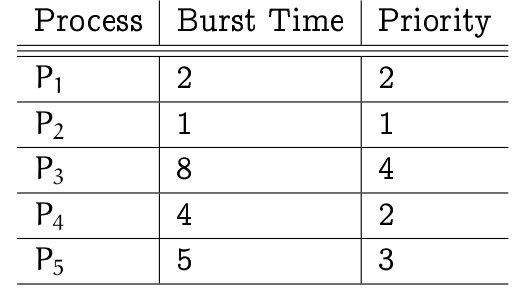
\includegraphics[scale=0.5]{ex-5_7.png} \\

The processes are assumed to have arrived in the order P1 , P2 , P3, P4 , P5 all at time 0.\\
\hspace{10mm}Draw four Gantt charts that illustrate the execution of these processes using the following scheduling algorithms: FCFS, SJF, nonpreemptive priority (a smaller priority number implies a higher priority), and RR (quantum = 1).
\textbf{ \\
\hspace{20mm} FCFS = 11233333333444455555 \\
\hspace{20mm} SJF \hspace{2mm} = 21144445555533333333 \\
\hspace{20mm} NPP \hspace{0.25mm} = 21144445555533333333\\
\hspace{20mm} RR \hspace{2.75mm} = 12345134534534535333 
}


\hspace{10mm}What is the turnaround time of each process for each of the scheduling algorithms in part a? \\
\hspace{20mm} \textbf{text} \\


\hspace{10mm}What is the waiting time of each process for each of these scheduling algorithms? \\
\hspace{20mm} \textbf{text} \\


\hspace{10mm}Which of the algorithms results in the minimum average waiting time (over all processes)? \\
\hspace{20mm} \textbf{text} \\



\subsubsection{5.10}
Which of the following scheduling algorithms could result in starvation?\\
\hspace{10mm}First-come, first-served\\
\hspace{20mm} \textbf{text} \\


\hspace{10mm}Shortest job first\\
\hspace{20mm} \textbf{text} \\


\hspace{10mm}Round robin\\
\hspace{20mm} \textbf{text} \\


\hspace{10mm}Priority\\
\hspace{20mm} \textbf{text} \\

\subsubsection{5.11}
Consider a variant of the RR scheduling algorithm where the entries in the ready queue are pointers to the PCBs. \\
\hspace{10mm}What would be the effect of putting two pointers to the same process in the ready queue?\\
\hspace{20mm} \textbf{text} \\


\hspace{10mm}What would be two major advantages and disadvantages of this scheme?\\
\hspace{20mm} \textbf{text} \\


\hspace{10mm}How would you modify the basic RR algorithm to achieve the same effect without the duplicate pointers?\\
\hspace{20mm} \textbf{text} \\


\subsubsection{5.12}
Consider a system running ten I/O-bound tasks and one CPU-bound task. Assume that the I/O-bound tasks issue an I/O operation once for every millisecond of CPU computing and that each I/O operation takes 10 milliseconds to complete. Also assume that the context-switching overhead is 0.1 millisecond and that all processes are long-running tasks. Describe is the CPU utilization for a round-robin scheduler when:
\\
\hspace{10mm}The time quantum is 1 millisecond\\
\hspace{20mm} \textbf{1/1,1 = 91 \%} \\


\hspace{10mm}The time quantum is 10 milliseconds\\
\hspace{20mm} \textbf{20/101.1+101 = 94 \%} \\

\subsubsection{5.16}
Explain the differences in how much the following scheduling algorithms discriminate in favor of short processes:\\
\hspace{20mm} \textbf{text} \\


\hspace{10mm}FCFS\\
\hspace{20mm} \textbf{ favor of when the tasks are dispatched} \\


\hspace{10mm}RR\\
\hspace{20mm} \textbf{Favor of short processes.} \\


\hspace{10mm}Multilevel feedback queues\\
\hspace{20mm} \textbf{Works like RR, but with a higher favor of shorter jobs.} \\



\vspace{10mm}
Discuss the most important parts from chapter 5, i.e. what worth including for the exam presentation titled: "Process Scheduling". Make a 10 keyword list for the topic. \\
Work on the following exercises and discuss the results

\subsubsection{5.4}
In this chapter, we discussed possible race conditions on various kernel data structures. Most scheduling algorithms maintain a run queue, which lists processes eligible to run on a processor. On multicore systems, there are two general options: (1) each processing core has its own run queue, or (2) a single run queue is shared by all processing cores. What are the advantages and disadvantages of each of these approaches?\\
\hspace{20mm} \textbf{text} \\

\subsubsection{5.5}
Consider the exponential average formula used to predict the length of the next CPU burst. What are the implications of assigning the following values to the parameters used by the algorithm? \\
\hspace{10mm}$\alpha$ = 0 and $\varsigma 0$ = 100 milliseconds \\
\hspace{20mm} \textbf{text} \\


\hspace{10mm}$\alpha$ = 0.99 and $\varsigma 0$ = 10 milliseconds\\
\hspace{20mm} \textbf{text} \\


\subsubsection{5.8}
The following processes are being scheduled using a preemptive, round-robin scheduling algorithm. Each process is assigned a numerical priority, with a higher number indicating a higher relative priority. In addition to the processes listed below, the system also has an idle task (which consumes no CPU resources and is identified as Pidle). This task has priority 0 and is scheduled whenever the system has no other availableprocesses to run. The length of a time quantum is 10 units. If a process is preempted by a higher-priority process, the preempted process is placed at the end of the queue. 
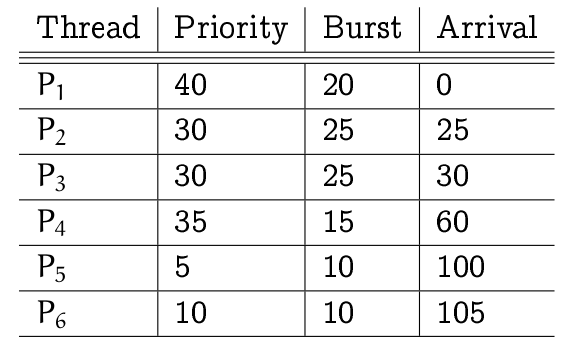
\includegraphics[scale=0.5]{ex-5_8.png} \\
Show the scheduling order of the processes using a Gantt chart.\\
\hspace{10mm}What is the turnaround time for each process?\\
 \textbf{
\hspace{20mm} p1 = 20 - 0 = 20\\
\hspace{20mm} p2 = 55 \\
\hspace{20mm} p3 = 60 \\
\hspace{20mm} p4 = 15 \\
\hspace{20mm} p5 = 20 \\
\hspace{20mm} p6 = 10 \\
} 


\hspace{10mm}What is the waiting time for each process?\\
\hspace{20mm} \textbf{
\hspace{20mm} p1 = 0\\
\hspace{20mm} p2 = 30 \\
\hspace{20mm} p3 = 35 \\
\hspace{20mm} p4 = 0 \\
\hspace{20mm} p5 = 10 \\
\hspace{20mm} p6 = 0 \\
} 


\hspace{10mm}What is the CPU utilization rate?\\
\hspace{20mm} \textbf{
105/120 = 87.5 \%
} \\

\subsubsection{5.13}
Consider a system implementing multilevel queue scheduling. What strategy can a computer user employ to maximize the amount of CPU time allocated to the user's process?\\
\hspace{20mm} \textbf{
test
} \\


\subsubsection{5.14}
Consider a preemptive priority scheduling algorithm based on dynamically changing priorities. Larger priority numbers imply higher priority. When a process is waiting for the CPU (in the ready queue, but not running), its priority changes at a rate $\alpha$ ; when it is running, its priority changes at a rate $\beta$ . All processes are given a priority of 0 when they enter the ready queue. The parameters $\alpha$ and $\beta$ can be set to give many different scheduling algorithms.\\

\hspace{10mm}What is the algorithm that results from $\beta$ > $\alpha$ > 0?\\
\hspace{20mm} \textbf{
	The one that is running is only getting high prioirty, therefor First Come First Serve.
} \\


\hspace{10mm}What is the algorithm that results from $\alpha$ < $\beta$ < 0?\\

\setlength\parindent{20mm} \textbf{
	The longer the process has been running the lower the prioiry, last in, first out.
} \\

\subsubsection{5.19}
Assume that two tasks A and B are running on a Linux system. The nice values of A and B are -5 and +5, respectively. Using the CFS scheduler as a guide, describe how the respective values of vruntime vary between the two processes given each of the following scenarios:\\
\hspace{10mm} Both A and B are CPU-bound.\\
\hspace{20mm} \textbf{
	text
} \\

\hspace{10mm} A is I/O-bound, and B is CPU-bound.\\
\hspace{20mm} \textbf{
	text
} \\

\hspace{10mm} A is CPU-bound, and B is I/O-bound.\\
\hspace{20mm} \textbf{
	text
} \\
\subsection{Lecture 4 - Exercise}
6.1 Race conditions are possible in many computer systems. Consider a banking system with two methods: deposit(amount) and withdraw(amount). These two methods are passed the amount that is to be deposited or withdrawn from a bank account. Assume that a husband and wife share a bank account and that concurrently the husband calls the withdraw() method and the wife calls deposit(). Describe how a race condition is possible and what might be done to prevent the race condition from occurring.\\

\textbf{
Deposit loads  amount of money\\
withdraw loads amount amount og money\\
Deposit saves\\
withdraw saves\\
therefor deposit is gone.
}
\\




6.2 The first known correct software solution to the critical-section problem for two processes was developed by Dekker. The two processes, P 0 and P 1 , share the following variables:
\begin{lstlisting}[frame=single]
boolean flag[2]; /* initially false */
int turn;
\end{lstlisting}
The structure of process P i ( i = 0 or 1) is shown in the Figure below; the other process is P j , ( j = 1 or 0). Prove that the algorithm satises all three requirements for the critical-section problem.\\
\begin{lstlisting}[frame=single]
do {
    flag[i] = true;
    while (flag[j]) {
        if (turn == j) {
            flag[i] = false;
            while (turn == j) {
                ; /* do nothing */
            }
            flag[i] = true;
        }
    }
    /* critical section */
    //Here we make it the other process turn
    turn = j;
    flag[i] = false;
    /* remainder section */
} while (true);

\end{lstlisting}

\subsubsection{6.4} 
Explain why implementing synchronization primitives by disabling interrupts is not appropriate in a single-processor system if the synchronization primitives are to be used in user-level programs.
\textbf{Because you can lock the user out, which means other process can't execute.}
\\
\subsubsection{6.5} 
Explain why interrupts are not appropriate for implementing synchronization primitives in multiprocessor systems.
\textbf{test}
\\
\subsubsection{6.6} 
The Linux kernel has a policy that a process cannot hold a spinlock while attempting to acquire a semaphore. Explain why this policy is in place.\\
\textbf{We risk that the spinlock is held for a long time, and its therefor better to use a mutex lock}
\\
\subsubsection{6.7}
Describe two kernel data structures in which race conditions are possible. Be sure to include a description of how a race condition can occur.\\
\textbf{•}
\\
\subsubsection{6.11}
Assume that a system has multiple processing cores. For each of the following scenarios, describe which is a better locking mechanism-a spinlock or a mutex lock where waiting processes sleep while waiting for the lock to become available:\\
The lock is to be held for a short duration.\\
\textbf{spinlock}\\
The lock is to be held for a long duration.\\
\textbf{mutex lock}\\
The thread may be put to sleep while holding the lock.\\
\textbf{You shouln't avoid using a lock in this case.}

\subsubsection{6.12}
Assume a context switch takes T time. Suggest an upper bound (in terms of T ) for holding a spin lock and that if the spin lock is held for any longer duration, a mutex lock (where waiting threads are put to sleep) is a better alternative.\\
\textbf{if the time in the lock is over t*2 then we should avoid using a spinlock.}
\subsubsection{6.19} Demonstrate that monitors and semaphores are equivalent insofar as they can be used to implement the same types of synchronization problems.\\
\textbf{Monitors has a condition that needs to be met while semaphores only has a counter the needs to be incremented or decremented.}

\subsubsection{6.22} Discuss the tradeoff between fairness and throughput of operations in the readers-writers problem. Propose a method for solving the readers-writers problem without causing starvation.\\
\textbf{
You can only have 1 writer per page, but unlimited readers.\\
Readers can have shared access, while writers have excusive access\\
}

\subsubsection{6.23} How does the signal() operation associated with monitors differ from the corresponding operation defined for semaphores?\\

\textbf{
If a monitor calls signal but no tasks are waiting nothing will happen. and if a tasks calls it just after it will go to the waiting state and wont be affected by that signal
}
\textbf{
When we signal with a semaphore we increment a counter, so if a process comes just after that is a slot open, but we risk the slot being closed.
}


\subsubsection{6.3}
The first known correct software solution to the $critical-section$ problem for n processes with a lower bound on waiting of $n-1$ turns was presented by Eisenberg and McGuire. \\
The processes share the following variables:

\begin{lstlisting}[frame=single]
enum pstate {idle, want_in, in_cs};
pstate flag[n];
int turn;
\end{lstlisting}
All the elements of flag are initially idle; the initial value of turn is immaterial (between 0 and n - 1 ). The structure of process Pi is shown in the Figure below. Prove that the algorithm satisfies all three requirements for the critical-section problem.\\

\begin{lstlisting}[frame=single]
do {
    while (true) {
    	-------------------------------------
    	// The process checks the states of all the other processes and checks if its idle
    	-------------------------------------
        flag[i] = want in;
        j = turn;
        while (j != i) {
            if (flag[j] != idle) {
            j = turn;
        } else {
            j = (j + 1) % n;
        }
        -------------------------------------
        checks again if all threads are idle and checks if any other threads and in cs
        -------------------------------------
        flag[i] = in cs;
        j = 0;
        while ( (j < n) && (j == i || flag[j] != in cs)) {
            j++;
        }
        if ( (j >= n) && (turn == i || flag[turn] == idle)) {
            break;
        }
        -------------------------------------
    }
    /* critical section */
    j = (turn + 1) % n;
    while (flag[j] == idle) {
        j = (j + 1) % n;
    }
    turn = j;
    flag[i] = idle;
    /* remainder section */
} while (true);
\end{lstlisting}

\subsubsection{6.9}
Consider how to implement a mutex lock using an atomic hardware instruction. Assume that the following structure defining the mutex lock is available:
\begin{lstlisting}[frame=single]
typedef struct {
    int available;
} lock;
\end{lstlisting}
where ( available $==$ 0 ) indicates the lock is available; a value of 1 indicates the lock is unavailable. Using this struct, illustrate how the following functions may be implemented using the test\_and\_set() and compare\_and\_swap() instructions.\\
void acquire(lock *mutex)\\
\textbf{
while mutex.int != 0 (
	if mutex.int == 0;(
	   mutex.int = 1;
	   )
	   )
}
void release(lock *mutex)\\
\textbf{mutex.int = 1;}
Be sure to include any initialization that may be necessary.\\
\subsubsection{6.14}
Consider the code example for allocating and releasing processes shown in the Figure below.
\begin{lstlisting}[frame=single]
#define MAX PROCESSES 255
int number of processes = 0;
 
/* the implementation of fork() calls this function */
int allocate process() {
    int new pid;
    if (number of processes == MAX PROCESSES) {
        return -1;
    } else {
        /* allocate necessary process resources */
        ++number of processes;
 
        return new pid;
    }
}
/* the implementation of exit() calls this function */
void release process() {
    /* release process resources */
    --number of processes;
}
\end{lstlisting}
Identify the race condition(s).
\textbf{because there a no lock, we can risk having 2 processes both accolate to many resources.} \\
Assume you have a mutex lock named mutex with the operations acquire() and release(). Indicate where the locking needs to be placed to prevent the race condi- tion(s). \\
\textbf{We'd place them lock and release just before and after the function.} \\
Could we replace the integer variable

\begin{lstlisting}[frame=single]
int number_of_processes = 0
\end{lstlisting}
with the atomic integer
\begin{lstlisting}[frame=single]
atomic_t number_of_processes = 0
\end{lstlisting}
to prevent the race condition(s)? \\
\textbf{nope. its not the int, its the function.}

\subsubsection{6.28}
6.28 Suppose we replace the wait() and signal() operations of monitors with a single con- struct await(B) , where B is a general Boolean expression that causes the process executing it to wait until B becomes true.
Write a monitor using this scheme to implement the readers-writers problem. b. Explain why, in general, this construct cannot be implemented efficiently.\\
\textbf{You need to check if there are either any active writers and any writers waiting.} \\
\textbf{That there only is 1 active writer and no readers can be started as they'd get a wrong value} \\

Why is it important for the scheduler to distinguish I/O-bound programs from CPU- bound programs?\\
\textbf{IO bound have more wait time, while CPU bound dont have much or any wait time.}
\subsubsection{6.8}
6.8 (modified) Describe how the compare and swap() (not described in detail in the lecture) instruction can be used to \\

to provide mutual exclusion \\
\textbf{Because the compare and swap function can only be used by one function} \\
to provide mutual exclusion that satisfies the bounded-waiting requirement. \\
\textbf{If we put the lock outside of the critical section it can cause some problems related to wait time}



\newpage
\subsection{Lecture 5 - Exercise}

\subsubsection{7.1} Consider the trafic deadlock depicted the Figure below (from the course book). 
\\
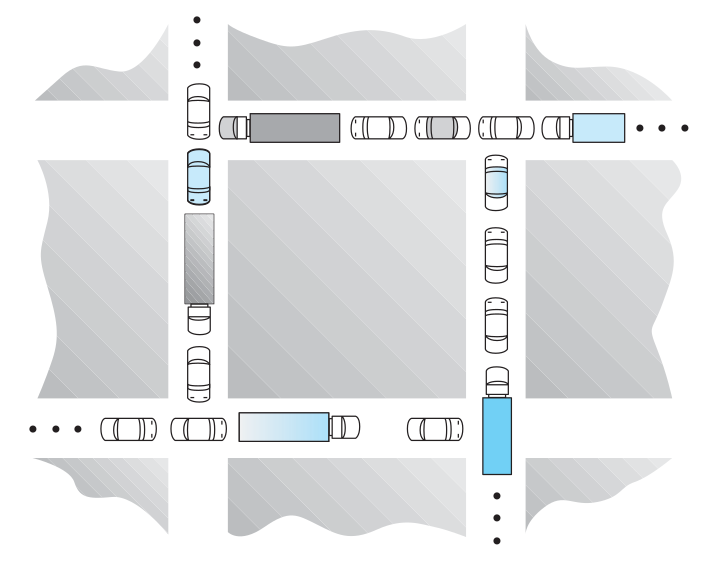
\includegraphics[scale=0.5]{ex-7_1.png}
\\
Show that the four necessary conditions for deadlock hold in this example.\\
State a simple rule for avoiding deadlocks in this system.\\
\textbf{mutual exclution \\
hold and wait\\
no premtion \\
no preemption \\
circular wait \\}
\vspace{10mm}
\textbf{A simple solution would be that you cant be in the intersection}

\subsubsection{7.2} 
Assume a multithreaded application uses only reader–writer locks for synchronization. Applying the four necessary conditions for deadlock, is deadlock still possible if multiple reader–writer locks are used?
\\
\textbf{Mutex excluion can be upheld becase writers have an exclusive lock, while readers use a shared lock.}
\\
\textbf{hold and wait, readers always wait for writers.}

\newpage

\subsubsection{7.3} The program example shown below doesn't always lead to deadlock. Describe what role the CPU scheduler plays and how it can contribute to deadlock in this program.
\begin{lstlisting}[frame=single]
/* thread one runs in this function */
void *do_work_one(void *param) {
    pthread_mutex_lock(&first mutex);
    pthread_mutex_lock(&second mutex);
    /**
     * Do some work
     */
    pthread_mutex_unlock(&second mutex);
    pthread_mutex_unlock(&first mutex);
    pthread_exit(0);
}
 
/* thread two runs in this function */
void *do work two(void *param) {
    pthread_mutex_lock(&second mutex);
    pthread_mutex_lock(&first mutex);
    /**
     * Do some work
     */
    pthread_mutex_unlock(&first mutex);
    pthread_mutex_unlock(&second mutex);
    pthread_exit(0);
}   
\end{lstlisting}
\textbf{If we get a interupt after the first lock has been acquired both threds will get a lock each, and the process with hold.}

\subsubsection{7.5} Compare the circular-wait scheme with the various deadlock-avoidance schemes (like the banker's algorithm) with respect to the following issues:\\
Runtime overheads\\
\textbf{circular-wait will be relativily cheap to run, while  deadlock-avoidance schemes and a lot mor expentive}\\
System throughput\\
\textbf{We can't say anything about that as its all about how the program is made.}

\subsubsection{7.9} Consider the version of the dining-philosophers problem in which the chopsticks are placed at the center of the table and any two of them can be used by a philosopher. Assume that requests for chopsticks are made one at a time. Describe a simple rule for determining whether a particular request can be satisfied without causing deadlock given the current allocation of chopsticks to philosophers.\\
\textbf{Both chopsticks have to be allocated at the same time or theres a risk of deadlocks.}



\subsubsection{7.10} Consider again the setting in the preceding question. Assume now that each philosopher requires three chopsticks to eat. Resource requests are still issued one at a time. Describe some simple rules for determining whether a particular request can be satisfied without causing deadlock given the current allocation of chopsticks to philosophers.\\
\textbf{Same.}



\subsubsection{7.12} Consider the following snapshot of a system: 
\\
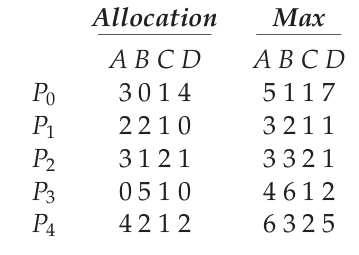
\includegraphics[scale=0.5]{ex-7_12.png}
\\
Using the banker's algorithm, determine whether or not each of the following states is unsafe. If the state is safe, illustrate the order in which the processes may complete. Otherwise, illustrate why the state is unsafe.\\
Available = (0, 3, 0, 1)\\
\begin{tabular}{|c|c|c|c|c|}
\hline 
• & allo & max & avail & need \\ 
\hline 
p1 & 3014 & 5117 & • & 2103 \\ 
\hline 
p2 & 2210 & 3211 & • & 1001 \\ 
\hline 
p3 & 3121 & 3321 & • & 0200 \\ 
\hline 
p4 & 0510 & 4612 & • & 4102 \\ 
\hline 
p5 & 4212 & 6325 & • & 2113 \\ 
\hline 
\end{tabular} \\
p2, p1, p3. and the last two will never be able to run, and therefor the sustem will be unable to run.
Available = (1, 0, 0, 2)\\






\subsubsection{7.15} 
A single-lane bridge connects the two Vermont villages of North Tunbridge and South Tunbridge. Farmers in the two villages use this bridge to deliver their produce to the neighboring town. The bridge can become deadlocked if both a northbound and a southbound farmer get on the bridge at the same time (Vermont farmers are stubborn and are unable to back up). Using semaphores, design an algorithm that prevents dead- lock. Initially, do not be concerned about starvation (the situation in which northbound farmers prevent southbound farmers from using the bridge, and vice versa).\\
\begin{lstlisting}
semaphore ok_to_access = 1;

Void enter_bridge(){
	okay_to_enter.wait();
};

Void exit_bridge(){
	okay_to_enter.signal();
};

\end{lstlisting}


\subsubsection{7.16} Modify your solution to Exercise 7.15 so that it is starvation-free.\\
\textbf{Add counter so more cant enter if there a people waiting}. \\




\subsubsection{7.6} In a real computer system, neither the resources available nor the demands of pro- cesses for resources are consistent over long periods (months). Resources break or are replaced, new processes come and go, new resources are bought and added to the sys- tem. If deadlock is controlled by the banker's algorithm, which of the following changes can be made safely (without introducing the possibility of deadlock), and under what circumstances?\\

Increase Available (new resources added)\\
\textbf{we can do this} \\
Decrease Available (resource permanently removed from system)\\
\textbf{This could make cause some problems.}\\

Increase Max for one process (the process needs or wants more resources than allowed).\\
\textbf{This could cause a deadlock }\\

Decrease Max for one process (the process decides it does not need that many resources)\\
\textbf{we can do that.} \\

Increase the number of processes\\
\textbf{It depends on the resources need. can go both ways.}\\

Decrease the number of processes\\
\textbf{It depends on the resources need. can go both ways.}\\



\subsubsection{7.7} Consider a system consisting of four resources of the same type that are shared by three processes, each of which needs at most two resources. Show that the system is deadlock-free.\\

\textbf{we have n+1. so there is always 1 process that can get 2, so no deadlocks can happen.} \\

\subsubsection{7.8} Consider a system consisting of m resources of the same type being shared by n processes. A process can request or release only one resource at a time. Show that the system is deadlock free if the following two conditions hold:\\
i.) The maximum need of each process is between 1 and m resources, and \\
ii.) The sum of all maximum needs is less than m + n\\





\subsubsection{7.13} Consider the following snapshot of a system: \\
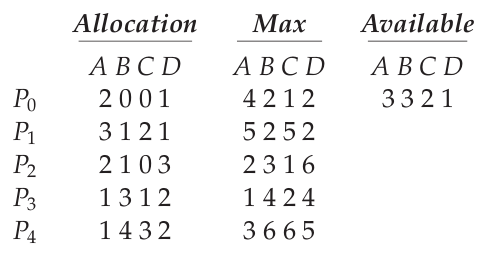
\includegraphics[scale=0.5]{ex-7_13.png} \\
Assume the Available vector being (A,B,C,D)=(3,3,2,1). Answer the following questions using the banker's algorithm:\\

Illustrate that the system is in a safe state by demonstrating an order in which the processes may complete.\\
p0, p2, p4, p1, p3.

If a request from process P1 arrives for (1, 1, 0, 0), can the request be granted immediately?\\
p0, p3, p4, p1, p2.

If a request from process P4 arrives for (0, 0, 2, 0), can the request be granted immediately?\\
deadlock.

\subsubsection{7.11} We can obtain the banker's algorithm for a single resource type from the general banker's algorithm simply by reducing the dimensionality of the various arrays by 1. Show through an example that we cannot implement the multiple-resource-type banker's scheme by applying the single-resource-type scheme to each resource type individually.



\newpage
\subsection{Lecture 6 - Exercise}
\subsubsection{8.1}
 Explain the difference between internal and external fragmentation. \\
external fragmentation - How much space is wasted between processes \\

internal fragmentation - How much space is wasted internally in a process \\

\subsubsection{8.2}
Consider the following process for generating binaries. A compiler is used to generate the object code for individual modules, and a linkage editor is used to combine multiple object modules into a single program binary. How does the linkage editor change the binding of instructions and data to memory addresses? What information needs to be passed from the compiler to the linkage editor to facilitate the memory binding tasks of the linkage editor? \\

\subsubsection{8.3}
Given five memory partitions of 100 KB, 500 KB, 200 KB, 300 KB, and 600 KB (in order), how would each of the first-fit, best-fit, and worst-fit algorithms place processes of 212 KB, 417 KB, 112 KB, and 426 KB (in order)? Which algorithm makes the most efficient use of memory? \\
\begin{tabular}{|c|c|c|c|c|c|}
\hline 
partitions & 100 & 500 & 200 & 300 & 600 \\ 
\hline 
first fit(fails for 4) & • & 1 & 3 & • & 2 \\ 
\hline 
best fit  & • & 2 & 3 & 1 & 4 \\ 
\hline 
worst fit(fails for 4) & • & 2 & • & 3 & 1 \\ 
\hline 
\end{tabular} 
\\
Best fit is generally the best \\
\subsubsection{8.4}
Most systems allow programs to allocate more memory to its address space during execution. Data allocated in the heap segments of programs are an example of such allocated memory. What is required to support dynamic memory allocation in the following schemes:
\\
\hspace{10mm}   contiguous memory allocation - \\
\hspace{10mm}	pure segmentation - \\
\hspace{10mm}	pure paging - Split the whole program up into smaller frames\\


\subsubsection{8.5}
external fragmentation\\
internal fragmentation\\
ability to share code across processes\\


\subsubsection{8.6}

\subsubsection{8.9}
\subsubsection{8.10}
\subsubsection{8.12}
\subsubsection{8.13}
\subsubsection{8.14}
\subsubsection{8.16}
\subsubsection{8.7}
\subsubsection{8.8}
Program binaries in many systems are typically structured as follows. Code is stored starting with a small fixed virtual address such as 0. The code segment is followed by the data segment that is used for storing the program variables. When the program starts executing, the stack is allocated at the other end of the virtual address space and is allowed to grow towards lower virtual addresses. What is the significance of the above structure for the following schemes:\\
\hspace{10mm} 1. contiguous-memory allocation \\

\hspace{15mm}  The stack wont be able to grow as it would cause collitions with other memory allocations \\


\hspace{10mm} 2. pure segmentation\\
\hspace{15mm} Insted af assign a whole address space we can assign small segments. \\

\hspace{10mm} 3. pure paging\\
\hspace{15mm} With pure paging we can allow the stack to become as big as we want it to. \\



\subsubsection{8.11}
Consider a computer system with a 32-bit logical address and 4-KB page size. The system supports up to 512 MB of physical memory. How many entries are there in each of the following?\\
\hspace{10mm}A conventional single-level page table?\\
\hspace{15mm}
\begin{equation}
2^{20} 
\end{equation}\\
\hspace{10mm}An inverted page table?
\hspace{15mm} \begin{equation}
2^{20/2}
\end{equation} \\





\subsubsection{8.15}
Consider the following segment table:\\
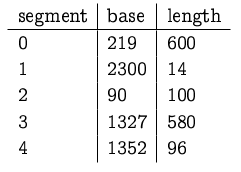
\includegraphics[scale=1]{ex-8-15.png}
\\
\begin{flushleft}

What are the physical addresses for the following logical addresses?
\end{flushleft}

\hspace{10mm}    0,430 - 430 + 219 = 649 \\
\hspace{10mm}    1,10 -  10 + 2300 = 2310\\
\hspace{10mm}    2,500 - connot be done \\
\hspace{10mm}    3,400 - 400 + 1327 = 1727\\
\hspace{10mm}    4,112 - connot be done \\
\subsubsection{8.17}
Consider the hierarchical paging scheme used by the VAX architecture. How many memory operations are performed when an user program executes a memory load op- eration?\\
\hspace{10mm} You use one operation to check the page table, and one for reading the page. \\
\hspace{15mm} maybe also one for getting the page? \\ 
\hspace{15mm} in total its 3\\

\subsubsection{8.8}
Compare the segmented paging scheme with the hashed page tables scheme for handling large address spaces. \\
\begin{flushleft}
Under what circumstances is one scheme preferable to the other?\\
\end{flushleft}
\hspace{10mm} With hashing it uses less space, but we get a longer runtime and there can be collisions \\

\newpage
\subsection{Lecture 7 - Exercise}

9.1
TLB miss with no page fault
	If the entry is not in the TLB but the page is already in memory

TLB miss and page fault
	Entry is not in TLB and is not in memory 

TLB hit and no page fault
	Its in TLB and in memory

TLB hit and page fault
	It's in TLB but not in memory
	Not possible

9.2
	1. It'll be blocked
	
	2. (Ready), it'll go to either blocked or continue running.
	
	3. It will keep running
	
9.3
	1. Every page is a page fault.
	
	2. Every working page is in memory so should be none or low
	
	3. 
		Ignore it
		Get more physical memory
		Replace pages more aggressively
9.4
	if two processes share a non changing variable and one of them changes it, and they fork.
	
	
9.5
	nope
	
9.8
	7, 2, 3, 1, 2, 5, 3, 4, 6, 7, 7, 1, 0, 5, 4, 6, 2, 3, 0 , 1
	LRU
	
	
	FIFO
		
	
	
	Optimal replacement
	
	11123456


9.9




















\newpage
\subsection{Lecture 9 - Exercise}
\subsubsection{10.1}
Consider a file system where a file can be deleted and its disk space Reclaimed while links to that file still exist. What problems may occur if a new file is created in the same storage area or with the same absolute path name? How can these problems be avoided?

\hspace{15mm} \textbf{The links will point to the same place, so some pointers may violates the permissions. which may do so an file is nor permitted to be executed, or users may be allowed to view it/not view it} \\

\subsubsection{10.2}
The open-file table is used to maintain information about files that are currently open. Should the operating system maintain a separate table for each user or just maintain one table that contains references to files that are being accessed by all users at the current time?\\
\hspace{15mm} \textbf{There has to be one universal file table so the OS wont have to cross reference to check if its safe to change files.} \\


If the same file is being accessed by two different programs or users, should there be separate entries in the open file table? \\
\hspace{15mm} \textbf{•} \\


\subsubsection{10.3}
What are the advantages and disadvantages of a system providing mandatory locks instead of providing advisory locks whose usage is left to the users' discretion? \\
\hspace{15mm} \textbf{•} \\



\subsubsection{10.4}
Provide examples of applications that typically access files according to the following methods: i.) Sequential, ii.) Random \\
\hspace{15mm} \textbf{•} \\


\subsubsection{10.5}
Some systems automatically open a file when it is referenced for the first time, and close the file when the job terminates. Discuss the advantages and disadvantages of this scheme as compared to the more traditional one, where the user has to open and close the file explicitly. \\
\hspace{15mm} \textbf{•} \\

\subsubsection{10.6}
 If the operating system were to know that a certain application is going to access the file data in a sequential manner, how could it exploit this information to improve performance? \\
\hspace{15mm} \textbf{It can preload data needed for the program to avoid load time.} \\


\subsubsection{10.7}
Give an example of an application that could benefit from operating system support for random access to indexed files.\\
\hspace{15mm} \textbf{ It's good for a database system. as it uses random read quite a lot. } \\


\subsubsection{11.2}
Contrast the performance of the three techniques for allocating disk blocks (contiguous, linked, and indexed) for both sequential and random file access.\\
\hspace{15mm} \textbf{contiguous sequential	- is good} \\
\hspace{15mm} \textbf{contiguous random	- Would work okay.} \\
\hspace{15mm} \textbf{linked sequential	- Quite bad, as we don't know where future links are.} \\
\hspace{15mm} \textbf{linked random		- Quite bad, as we don't know where future links are. } \\
\hspace{15mm} \textbf{indexed sequential-  } \\
\hspace{15mm} \textbf{indexed random	- } \\


\subsubsection{11.4}
Consider a system where free space is kept in a free-space list.\\
\hspace{10mm}	Suppose that the pointer to the free-space list is lost. Can the system reconstruct the free-space list? Explain your answer.\\
\hspace{15mm} \textbf{We'll have to search the entire file structure to find free space and re link them.} \\


\hspace{10mm}Consider a file system similar to the one used by UNIX with indexed allocation. How many disk I/O operations might be required to read the contents of a small local file at /a/b/c? Assume that none of the disk blocks is currently being cached.\\
\hspace{15mm} \textbf{•} \\

\hspace{10mm}Suggest a scheme to ensure that the pointer is never lost as a result of memory failure.\\
\hspace{15mm} \textbf{•} \\



\subsubsection{11.5}
Some file systems allow disk storage to be allocated at different levels of granularity. For instance, a file system could allocate 4 KB of disk space as a single 4-KB block or as eight 512-byte blocks. How could we take advantage of this exibility to improve performance?
\\
\hspace{15mm} \textbf{•} \\

What modifications would have to be made to the freespace management scheme in order to support this feature?\\
\hspace{15mm} \textbf{•} \\


\subsubsection{11.7}
Consider a file system on a disk that has both logical and physical block sizes of 512 bytes. Assume that the information about each file is already in memory. For each of the three allocation strategies (contiguous, linked, and indexed), answer these questions:
\\
\hspace{10mm}How is the logical-to-physical address mapping accomplished in this system? (For the indexed allocation, assume that a file is always less than 512 blocks long.)
\\
\hspace{15mm} \textbf{•} \\




\hspace{10mm}If we are currently at logical block 10 (the last block accessed was block 10) and want to access logical block 4, how many physical blocks must be read from the disk?
\\
\hspace{15mm} \textbf{•} \\


\subsubsection{11.9}
Fragmentation on a storage device could be eliminated by decompaction of the information. Typical disk devices do not have relocation or base registers (such as are used when memory is to be compacted), so how can we relocate files? Give three reasons why recompacting and relocation of files often are avoided.\\
\hspace{15mm} \textbf{We can loose data when we move data, we can loose some of the pointers, } \\

\subsubsection{11.11}
Explain why logging metadata updates ensures recovery of a file system after a file system crash.\\
\hspace{15mm} \textbf{•} \\




\newpage
\subsection{Lecture 10 - Exercise}
\subsubsection{12.1} 
None of the disk-scheduling disciplines, except FCFS, is truly fair (starvation may occur). \\

\hspace{10mm} 	Explain why this assertion is true.\\
\hspace{15mm} \textbf{Because it will load things in the order they are requested.} \\


\hspace{10mm} 	Describe a way to modify algorithms such as SCAN to ensure fairness.\\
\hspace{15mm} \textbf{By having it jump all the way back to the start and read from the beginning the end.} \\


\hspace{10mm} 	Explain why fairness is an important goal in a time-sharing system.\\
\hspace{15mm} \textbf{•} \\


\hspace{10mm} 	Give three or more examples of circumstances in which it is important that the operating system be unfair in serving I/O requests.\\
\hspace{15mm} \textbf{•} \\




\subsubsection{12.2} Explain why SSDs often use a FCFS disk scheduling algorithm.\\
\hspace{15mm} \textbf{They don't have no seek time.} \\


\subsubsection{12.3} Suppose that a disk drive has 5000 cylinders, numbered 0 to 4999. The drive is currently serving a request at cylinder 2150, and the previous request was at cylinder 1805. The queue of pending requests, in FIFO order, is:\\

2069, 1212, 2296, 2800, 544, 1618, 356, 1523, 4965, 3681.  \\

Starting from the current head position, what is the total distance (in cylinders) that the disk arm moves to satisfy all the pending requests for each of the following disk-scheduling algorithms? \\


\hspace{10mm} 	FCFS     \\
\hspace{15mm} \textbf{13011} \\

\hspace{10mm} 	SSTF    \\
\hspace{15mm}\textbf{7586} \\

\hspace{10mm} 	SCAN    \\
\hspace{15mm}\textbf{7494} \\

\hspace{10mm} 	LOOK    \\
\hspace{15mm}\textbf{7424} \\

\hspace{10mm} 	C-SCAN  \\ 
\hspace{15mm}\textbf{9994} \\

\hspace{10mm} 	C-LOOK  \\
\hspace{15mm}\textbf{•} \\
	
	
\subsubsection{12.6} Describe some advantages and disadvantages of using SSDs as a caching tier and as a disk drive replacement compared to a system with just magnetic disks. \\
\hspace{15mm}\textbf{SSD low seek time, and high speed} \\

\hspace{15mm}\textbf{Disk drives, high seek time, and low speed} \\

\subsubsection{12.8} Requests are not usually uniformly distributed. For example, we can expect a cylinder containing the file-system metadata to be accessed more frequently than a cylinder containing only files.\\ 

\hspace{10mm} Suppose you know that 50 percent of the requests are for a small, fixed number of cylinders. \\

\hspace{10mm} Would any of the scheduling algorithms discussed in this chapter be particularly good for this case? Explain your answer. \\
\hspace{15mm}\textbf{Best for seek time, SSTF, but may cause starvation} \\
\hspace{15mm}\textbf{So C-look may be better.} \\

\hspace{10mm} Propose a disk-scheduling algorithm that gives even better performance by taking advantage of this "hot spot" on the disk \\
\hspace{15mm}\textbf{Using SSTF in the Hot Spot, and else use look, or C-look.} \\


\subsubsection{12.9} Consider a RAID Level 5 organization comprising five disks, with the parity for sets of four blocks on four disks stored on the fifth disk. How many blocks are accessed in order to perform the following?\\
\hspace{10mm} 	A write of one block of data\\
\hspace{15mm}\textbf{2 Block. what you're writing + parity(1)} \\
\hspace{10mm} 	A write of seven continuous blocks of data\\
\hspace{15mm}\textbf{9 Block. what you're writing + parity(2)} \\


\subsubsection{12.10} Compare the throughput achieved by a RAID Level 5 organization with that achieved by a RAID Level 1 organization for the following: \\
\hspace{10mm} 	Read operations on single blocks \\
\hspace{15mm} \textbf{Same} \\
\hspace{10mm} 	Read operations on multiple contiguous blocks \\
\hspace{15mm} \textbf{4x} \\

\subsubsection{12.12} Assume that you have a mixed configuration comprising disks organized as RAID Level 1 and as RAID Level 5 disks. Assume that the system has flexibility in deciding which disk organization to use for storing a particular file. Which files should be stored in the RAID Level 1, and which in the raid level 5.\\
\hspace{15mm} \textbf{Active files should be in raid level 5, and cold storage should be raid level 1.} \\


\subsubsection{12.14} Discuss the relative advantages and disadvantages of sector sparing and sector slipping.\\
\hspace{15mm} \textbf{Sector sparing may result in unexpected delay due to higher seek time.} \\
\hspace{15mm} \textbf{Sector slipping will result in higher performance as you wont have to go elsewhere for a different sector.} \\

\subsubsection{13.1} When multiple interrupts from different devices appear at about the same time, a priority scheme could be used to determine the order in which the interrupts would be serviced. Discuss what issues need to be considered in assigning priorities to different interrupts. \\
\hspace{15mm} \textbf{Generally Hardware should have higher interrupts. and devices with real time constraints should have higher priority.} \\


\subsubsection{13.2} What are the advantages and disadvantages of supporting memory-mapped I/O to device-control registers? \\
\hspace{15mm} \textbf{•} \\


\subsubsection{13.3} Consider the following I/O scenarios on a single-user PC.\\
\hspace{10mm} 	A mouse used with a graphical user interface \\
\hspace{15mm} \textbf{interrupt-driven} \\

\hspace{10mm} 	A tape drive on a multitasking operating system (assume no device preallocation is available) \\
\hspace{15mm} \textbf{spooling, as the tape drive has a high seek time.} \\

\hspace{10mm} 	A disk drive containing user files \\
\hspace{15mm} \textbf{Caching  } \\

\hspace{10mm} 	A graphics card with direct bus connection, accessible through memory-mapped I/O \\
\hspace{15mm} \textbf{ none of the designs are needed, and polled and interrupt will be used for the input path.} \\

\hspace{10mm} 	For each of these I/O scenarios, would you design the operating system to use buffering, spooling, caching, or a combination? Would you use polled I/O, or interrupt-driven I/O? Give reasons for your choices. \\
\hspace{15mm} \textbf{•} \\



\subsubsection{13.4} In most multiprogrammed systems, user programs access memory through virtual addresses, while the operating system uses raw physical addresses to access memory. What are the implications of this design on the initiation of I/O operations by the user program and their execution by the operating system? \\
\hspace{15mm} \textbf{ • } \\



\subsubsection{13.5} What are the various kinds of performance overheads associated with servicing an interrupt?\\
\hspace{15mm} \textbf{ saving, Swapping, and restoring the process state } \\



\subsubsection{13.6} Describe three circumstances under which blocking I/O should be used. Describe three circumstances under which non-blocking I/O should be used. Why not just implement non-blocking I/O and have processes busy-wait until their device is ready?\\
\hspace{15mm} \textbf{ Blocking is when waiting for one specifik event..} \\

\hspace{15mm} \textbf{ non-blocking is when you wait for multiple events, and multiple threads are waiting.} \\

\hspace{15mm} \textbf{ Threads could be in a starvation state. } \\


\subsubsection{12.4} Elementary physics states that when an object is subjected to a constant acceleration a , the relationship between distance d and time t is given by d = (1/2)at2 . Suppose that, during a seek, the disk in Exercise 12.3 accelerates the disk arm at a constant rate for the first half of the seek, then decelerates the disk arm at the same rate for the second half of the seek. Assume that the disk can perform a seek to an adjacent cylinder in 1 millisecond and a full-stroke seek over all 5000 cylinders in 18 milliseconds.\\
\hspace{10mm} 	The distance of a seek is the number of cylinders that the head moves. Explain why the seek time is proportional to the square root of the seek distance.\\
\hspace{15mm} 
\begin{equation}
t = \sqrt{(1/2)a*d}
\end{equation} \\



\hspace{10mm} 	Write an equation for the seek time as a function of the seek distance. This equation should be of the form t = x + y √ L , where t is the time in milliseconds and L is the seek distance in cylinders.\\
\hspace{15mm} \textbf{return math.sqrt((1/2)a*d)} \\
	
\hspace{10mm} 	Calculate the total seek time for each of the schedules in Exercise 12.3. Determine which schedule is the fastest (has the smallest total seek time). \\
\hspace{15mm} \textbf{•} \\

	
	
\hspace{10mm} 	The percentage speedup is the time saved divided by the original time. What is the percentage speedup of the fastest schedule over FCFS? \\
\hspace{15mm} \textbf{•} \\





\subsubsection{12.7} Compare the performance of C-SCAN and SCAN scheduling, assuming a uniform distribution of requests. Consider the average response time (the time between the arrival of a request and the completion of that request's service), the variation in response time, and the effective bandwidth. How does performance depend on the relative sizes of seek time and rotational latency? \\
\hspace{15mm} \textbf{•} \\




\subsubsection{12.13} The reliability of a hard-disk drive is typically described in terms of a quantity called mean time between failures (MTBF). Although this quantity is called a "time", the MTBF actually is measured in drivehours per failure. \\
\hspace{10mm} 	If a system contains 1000 drives, each of which has a 750,000-hour MTBF, which of the following best describes how often a drive failure will occur in that disk farm: once per thousand years, once per century, once per decade, once per year, once per month, once per week, once per day, once per hour, once per minute, or once per second? \\
\hspace{15mm} \textbf{•} \\

\hspace{10mm} 	Mortality statistics indicate that, on the average, a U.S. resident has about 1 chance in 1000 of dying between ages 20 and 21 years. Deduce the MTBF hours for 20 year olds. Convert this figure from hours to years. What does this MTBF tell you about the expected lifetime of a 20 year old? \\
\hspace{15mm} \textbf{•} \\

\hspace{10mm} 	The manufacturer guarantees a 1-million-hour MTBF for a certain model of disk drive. What can you conclude about the number of years for which one of these drives is under warranty?\\
\hspace{15mm} \textbf{•} \\




\subsubsection{12.15} Discuss the reasons why the operating system might require accurate information on how blocks are stored on a disk. How could the operating system improve file system performance with this knowledge? \\
\hspace{15mm} \textbf{•} \\



\subsubsection{13.7} Typically, at the completion of a device I/O, a single interrupt is raised and appropriately handled by the host processor. In certain settings, however, the code that is to be executed at the completion of the I/O can be broken into two separate pieces. The first piece executes immediately after the I/O completes and schedules a second interrupt for the remaining piece of code to be executed at a later time. What is the purpose of using this strategy in the design of interrupt handlers? \\
\hspace{15mm} \textbf{•} \\





\subsubsection{13.8} Some DMA controllers support direct virtual memory access, where the targets of I/O operations are specified as virtual addresses and a translation from virtual to physical address is performed during the DMA. How does this design complicate the design of the DMA controller? What are the advantages of providing such a functionality?\\
\hspace{15mm} \textbf{ The DMA needs to be aware of the page table. and the DMA needs to be able to locate the memory. and this make things much simpler on a application level.} \\

\subsection{Lecture 11 - Exercise}

\subsubsection{16.1} Describe the three types of traditional virtualization. \\
\hspace{10mm} \textbf{type 0 - Hardware-based solutions that provide support for virtual machine creation and management via firmware.} \\
\hspace{10mm} \textbf{type 1 - Operating-system-like software built to provide
virtualization} \\
\hspace{10mm} \textbf{type 3 - Applications that run on standard operating systems but provide VMM features to guest operating systems} \\


16.2 Describe the four virtualization-like execution environments and why they are not “true” virtualization. \\
\hspace{10mm} \textbf{Programming-environment virtualization - VMMs do not virtualize real
hardware but instead create an optimized virtual system} \\
\hspace{10mm} \textbf{Emulators – Allow applications written for one hardware environment to
run on a very different hardware environment, such as a different type of
CPU} \\
\hspace{10mm} \textbf{Paravirtualization - Technique in which the guest operating system is
modified to work in cooperation with the VMM to optimize performance} \\
\hspace{10mm} \textbf{Application containment - Not virtualization at all but rather provides
virtualization-like features by segregating applications from the operating
system, making them more secure, manageable} \\



16.3 Describe four benefits of virtualization. \\
\hspace{10mm} \textbf{Host system is protected from virus and the likes from the virtual machine.} \\


\hspace{10mm} \textbf{Live migration} \\


\hspace{10mm} \textbf{Templating} \\


\hspace{10mm} \textbf{Snapshots} \\


\hspace{10mm} \textbf{Cost and performance} \\

\hspace{10mm} \textbf{We can run multiple operating systems on the same set of hardware.} \\

\hspace{10mm} \textbf{Lower system admin, and } \\




16.4 Why can VMM s not implement trap-and-emulate-based virtualization on some CPU s? Lacking the ability to trap-and-emulate, what method can a VMM use to implement virtualization? \\
\hspace{10mm} \textbf{because some cpu can't separate privilege and non-privilege operations.} \\
\hspace{10mm} \textbf{Software emulate it, but this causes some overhead.} \\

16.5 What hardware assistance for virtualization can be provided by modern CPU s?\\
\hspace{10mm} \textbf{•} \\


16.6 Why is live migration possible in virtual environments but much less possible for a native operating system?\\
\hspace{10mm} \textbf{} \\



\subsection{Lecture 12 - Exercise}

\subsubsection{14.2} The access-control matrix could be used to determine whether a process can switch from, say, domain A to domain B and enjoy the access privileges of domain B. Is this approach equivalent to including the access privileges of domain B in those of domain A? 
\\ \hspace{10mm} \textbf{It's the same permissions} \\


\subsubsection{14.5} Discuss the strengths and weaknesses of implementing an access matrix using access lists that are associated with objects. 
\\ \hspace{10mm} \textbf{Its file based and not whole system based so its therefore more flexible., but the weakness is also that its does so there is way more book keeping} \\



\subsubsection{14.6} Discuss the strengths and weaknesses of implementing an access matrix using capabilities that are associated with domains. 
\\ \hspace{10mm} \textbf{Faster access, and more flexible on the individual objects} \\


\subsubsection{14.9} What is the need-to-know principle? Why is it important for a protection system to adhere to this principle?
\\ \hspace{10mm} \textbf{That you should only be able to see files if you have access to them. and by that protect the file system.} \\


\subsubsection{14.12} How are the access-matrix facility and the role-based access-control facility similar? How do they differ?
\\ \hspace{10mm} \textbf{matrix is more binary while role based is read, write, execute and so on.} \\


\subsubsection{14.13} How does the principle of least privilege aid in the creation of protection systems?
\\ \hspace{10mm} \textbf{That the user only have minimal access so they can do the job, but wont be able to damage the system both intensionally and unintentionally. } \\


\subsubsection{15.1} Buffer-overflow attacks can be avoided by adopting a better programming methodology or by using special hardware support. Discuss these solutions.
\\ \hspace{10mm} \textbf{bounds checking, sanitize your data, or set hardware limits} \\


\subsubsection{15.2} A password may become known to other users in a variety of ways. Is there a simple method for detecting that such an event has occurred? Explain your answer.
\\ \hspace{10mm} \textbf{Timestamp based to see when you where last logged in.} \\


\subsubsection{15.3} What is the purpose of using a "salt" along with the user-provided password? Where should the "salt" be stored, and how should it be used?
\\ \hspace{10mm} \textbf{•} \\


\subsubsection{15.4} The list of all passwords is kept within the operating system. Thus, if a user manages to read this list, password protection is no longer provided. Suggest a scheme that will avoid this problem. (Hint: Use different internal and external representations.)
\\ \hspace{10mm} \textbf{Hashing, 2 factor, biometric, limit access to hardware, limit access to the password folder.} \\



\subsubsection{15.9} Make a list of six security concerns for a bank's computer system. For each item on your list, state whether this concern relates to physical, human, or operating-system security.
\\ \hspace{10mm} \textbf{social engineering - human} 
\\ \hspace{10mm} \textbf{phishing - human} 
\\ \hspace{10mm} \textbf{Brute force - human} 


\subsubsection{15.10} What are two advantages of encrypting data stored in the computer system?
\\ \hspace{10mm} \textbf{Other people can't access it. encrypted data is also protected by the operating system.} \\



\subsubsection{15.12} Compare symmetric and asymmetric encryption schemes, and discuss under what circumstances a distributed system would use one or the other.
\\ \hspace{10mm} \textbf{1 key, vs 2 key., and in the distributed system you would use 2 key system} \\




\subsubsection{14.10} Discuss which of the following systems allow module designers to enforce the need-to-know principle. a. The MULTICS ring protection scheme b. JVM's stack-inspection scheme
\\ \hspace{10mm} \textbf{Ring protection does not hold this as it as you get more access than you should due to the way the ring protection scheme works.} \\
   \hspace{10mm} \textbf{You have access to what's below you on the stack so it'll give you more than need to know access} \\


\subsubsection{14.11} Describe how the Java protection model would be sacrificed if a Java program were allowed to directly alter the annotations of its stack frame.
\\ \hspace{10mm} \textbf{You can skip the access block and therefore break the security.} \\



\subsubsection{15.5} An experimental addition to UNIX allows a user to connect a watchdog program to a file. The watchdog is invoked whenever a program requests access to the file. The watchdog then either grants or denies access to the file. Discuss pros and cons of using watchdogs for security.
\\ \hspace{10mm} \textbf{It adds a layer more of security to the file. the problem with watchdogs is that it can be high bottlenecked if its badly implemented.} \\


\subsubsection{15.11} What commonly used computer programs are prone to man-in-the-middle attacks? Discuss solutions for preventing this form of attack.
\\ \hspace{10mm} \textbf{Any program that uses internet.} \\



\subsubsection{15.13} Why doesn't $D_{kd,N}(E_{ke,N}(m)) $ provide authentication of the sender? To what uses can such an encryption be put?
\\ \hspace{10mm} \textbf{first encrypt with your private key, then with theirs public key.} \\



\subsubsection{15.14} Discuss how the asymmetric encryption algorithm can be used to achieve the following goals.\\
Authentication: the receiver knows that only the sender could have generated the message.
\\ \hspace{10mm} \textbf{senders private key key} \\
Secrecy: only the receiver can decrypt the message.
\\ \hspace{10mm} \textbf{receivers public key} \\
Authentication and secrecy: only the receiver can decrypt the message, and the receiver knows that only the sender could have generated the message.
\\ \hspace{10mm} \textbf{first my private, then their public key.} \\


\end{document}
